\chapter{Le détecteur Compact Muon Solenoid (CMS)}
\renewcommand\chapterillustration{CMS/cms.jpeg}
\ThisULCornerWallPaper{1}{\chapterillustration}
\minitoc

\lettrine[lines=4, slope=-0.5em]{C}{e} chapitre décrit le détecteur CMS et les sous-détecteurs qui le compose, suivi d'une discussion sur le système de déclenchement. Il décrit également certaines des mises à niveaux qui se dérouleront durant les \textit{Long Shut Down} LS2 et LS3 afin de se préparer à l'augmentation de la luminosité et de l'empilement qui en découle.

\section{Le détecteur Solénoïde compact à muons (CMS)}
Le détecteur Solénoïde compact à muons abrégé en CMS (pour Compact Muon Solenoid) est avec ATLAS une expérience généraliste qui a comme buts majeurs :

\begin{itemize}[label=$\bullet$]
	\item \textbf{La recherche du boson de Higgs : } Lors de la conception de CMS dans les années 1990, la détection du boson de Higgs à été prise comme référence afin de tester les performances du design du détecteur. Ce but à été réalisé avec la découverte d'une particule compatible avec le boson de Higgs le 4 juillet 2012.
	\item \textbf{Confirmer et préciser les mesures de la physique du Modèle Standard : } Des mesures de précisions dans des domaines tels que la QCD, le couplage électrofaible, et la physique des saveurs pourraient donner des indications d'une physique au-delà du Modèle Standard.
	\item \textbf{La recherche de signes de physique au-delà du Modèle Standard : }CMS permet la recherche de particules supersymétriques ou de nouveaux bosons vecteurs massifs ($Z'$) ou encore la recherche de dimensions supplémentaires par exemple.
	\item \textbf{Étudier les collisions d'ions lourds.}
\end{itemize}

Afin de répondre à ces objectifs, le "Technical Design Report" (TDR) \cite{Bayatian:922757} a fixé le cahier des charges et les caractéristiques essentielles du détecteur CMS, à savoir :
\begin{itemize}[label=$\bullet$]
	\item Une bonne identification des muons et une bonne résolution en impulsion sur une vaste gamme d'impulsion pour la région $|\eta|<2.5$, une bonne résolution en masse pour les dimuons ($\approx 1\%$ à 100GeV/c$^{2}$) et la capacité à déterminer de manière certaine la charge des muons d'impulsion $p<$ 1TeV/c.
	\item Une bonne résolution en impulsion pour les particules chargées ainsi qu'une bonne efficacité de reconstruction dans le trajectographe interne (inner tracker). Un déclenchement et un étiquettage efficace pour les jets venant de quarks $\tau$ et $b$, ce qui requiert un détecteur à pixels proche du point d'interaction.
	\item Une bonne résolution pour l'énergie électromagnétique, et une bonne résolution en masse pour les diphotons et dielectrons  ($\approx 1\%$ à 100GeV/c$^{2}$), une grande couverture géométrique ($|\eta|<2.5$), une mesure de la direction des photons et/ou une localisation correcte du vertex primaire d'interaction ainsi qu'une bon rejet des $\pi_{0}$ et une isolation des photons et letptons efficace à haute luminosité.
	\item une bonne résolution en masse des dijets et une bonne résolution en masse de l'énergie transverse manquante $E_{T}^{miss}$. Ceci requiert un calorimètre hadronique hermétique de très grande couverture géométrique ($|\eta|<5$) et une fine segmentation latérale ($\Delta\eta\times\Delta\phi<0.1\times0.1$)
\end{itemize} 

\subsection{Système de coordonnées conventionnel}
Le système de coordonnées utilisé dans CMS est un repère cartésien $\left(O,\vec{x},\vec{y},\vec{z}\right)$ où $O$ est l'origine du repère et coïncide avec le point nominal d'interaction (IP) qui est le centre du détecteur. Le système de coordonnée est déterminé par l'axe $z$ qui est défini comme étant parallèle et dans la même direction que le faisceau allant dans le sens anti-horaire vue de dessus. L'axe $x$ pointe vers le centre du collisionneur LHC. L'axe $y$ est orthogonal au plan $xz$ et pointe vers le haut. CMS possédant une symétrie cylindrique, le repère $\left(O,\vec{r},\vec{\phi},\vec{z}\right)$ est souvent utilisé. $z$ correspond à la distance entre le plan perpendiculaire à l'axe du faisceau (appelé plan transverse) passant par le point considéré et l'origine $O$ du repère; $\phi$ est mesuré par rapport à l'axe $\vec{x}$ dans le plan $xy$ (angle d'émission par rapport à l'axe du faisceau) et $r=\sqrt{x^2+y^2}$. L'angle polaire $\theta$ est définit par rapport à $z$. Un troisième type de coordonnées, utilisant le fait que les particules produite au LHC sont relativistes, est également utilisé. En décomposant l'impulsion de la particule en une composante transverse et longitudinale $p=p_{T}+p_{L}=\sqrt{p_{x}^{2}+p_{y}^{2}}+p_{z}$ :
\begin{equation}
( E/c)^{2}=(mc)^{2}+p_{T}^{2}+p_{L}^{2}\Longrightarrow ( E/c)^{2}-p_{L}^{2}=(mc)^{2}+p_{T}^{2}\Longrightarrow  \begin{cases}
\left( E/c \right)=\sqrt{\left( mc \right)^{2}+p_{T}^{2}}\cosh(y) \\
p_{L}=\sqrt{\left( mc \right)^{2}+p_{T}^{2}}\sinh(y)
\end{cases}
\end{equation}
%qu'il est possible de réécrire comme :
%\begin{equation}
%\left( E/c \right)=\sqrt{\left( mc \right)^{2}+p_{T}^{2}}\cosh(y), p_{L}=\sqrt{\left( mc \right)^{2}+p_{T}^{2}}\sinh(y)
%\end{equation}
avec $y$ un paramètre appelé rapidité. En remarquant que $p_{l}=p_{z}=p\cos(\theta)$ et en faisant le développement de $E=\sqrt{m^{2}c^{4}+p^{2}c^{2}}$:
\begin{equation}
y=\arctan\left(\frac{p_{l}c}{E}\right)=\frac{1}{2}\log\left(\frac{E+p_{l}c}{E-p_{l}c}\right)=\frac{1}{2}\log\left(\frac{\cos^2 \theta/2+\cdots}{\sin^2 \theta/2+\cdots}\right)\backsimeq-\log\tan\left(\frac{\theta}{2}\right)=\eta
\end{equation}
%en remarquant que $p_{l}=p_{z}=p\cos(\theta)$ et en faisant le développement de $E=\sqrt{m^{2}c^{4}+p^{2}c^{2}}$
%\begin{equation}
%y=\frac{1}{2} \log\left(\frac{E+p_{l}c}{E-p_{l}c}\right)=\frac{1}{2}\log\left(\frac{\cos^2 %\theta/2+m^{2}c^{2}/4p^{2}+\cdots}{\sin^2 %\theta/2+m^{2}c^{2}/4p^{2}+\cdots}\right)\backsimeq-\log\tan\left(\frac{\theta}{2}\right)=\eta
%\end{equation}
$\eta$ est appellé pseudo-rapidité. On utilise donc le repère $\left(O,\vec{r},\vec{\eta},\vec{\phi}\right)$ pour décrire la géométrie de CMS.

\subsection{Description générale de CMS}
Le détécteur CMS se trouve dans une caverne situé au point 5 (P5) du LHC, proche du village de Cessy en France. La construction de CMS s'est effectué en surface et par tranches autonomes afin de réduire le temps et les coûts nécessaires à sa construction.
\marginpar
{
	\centering
	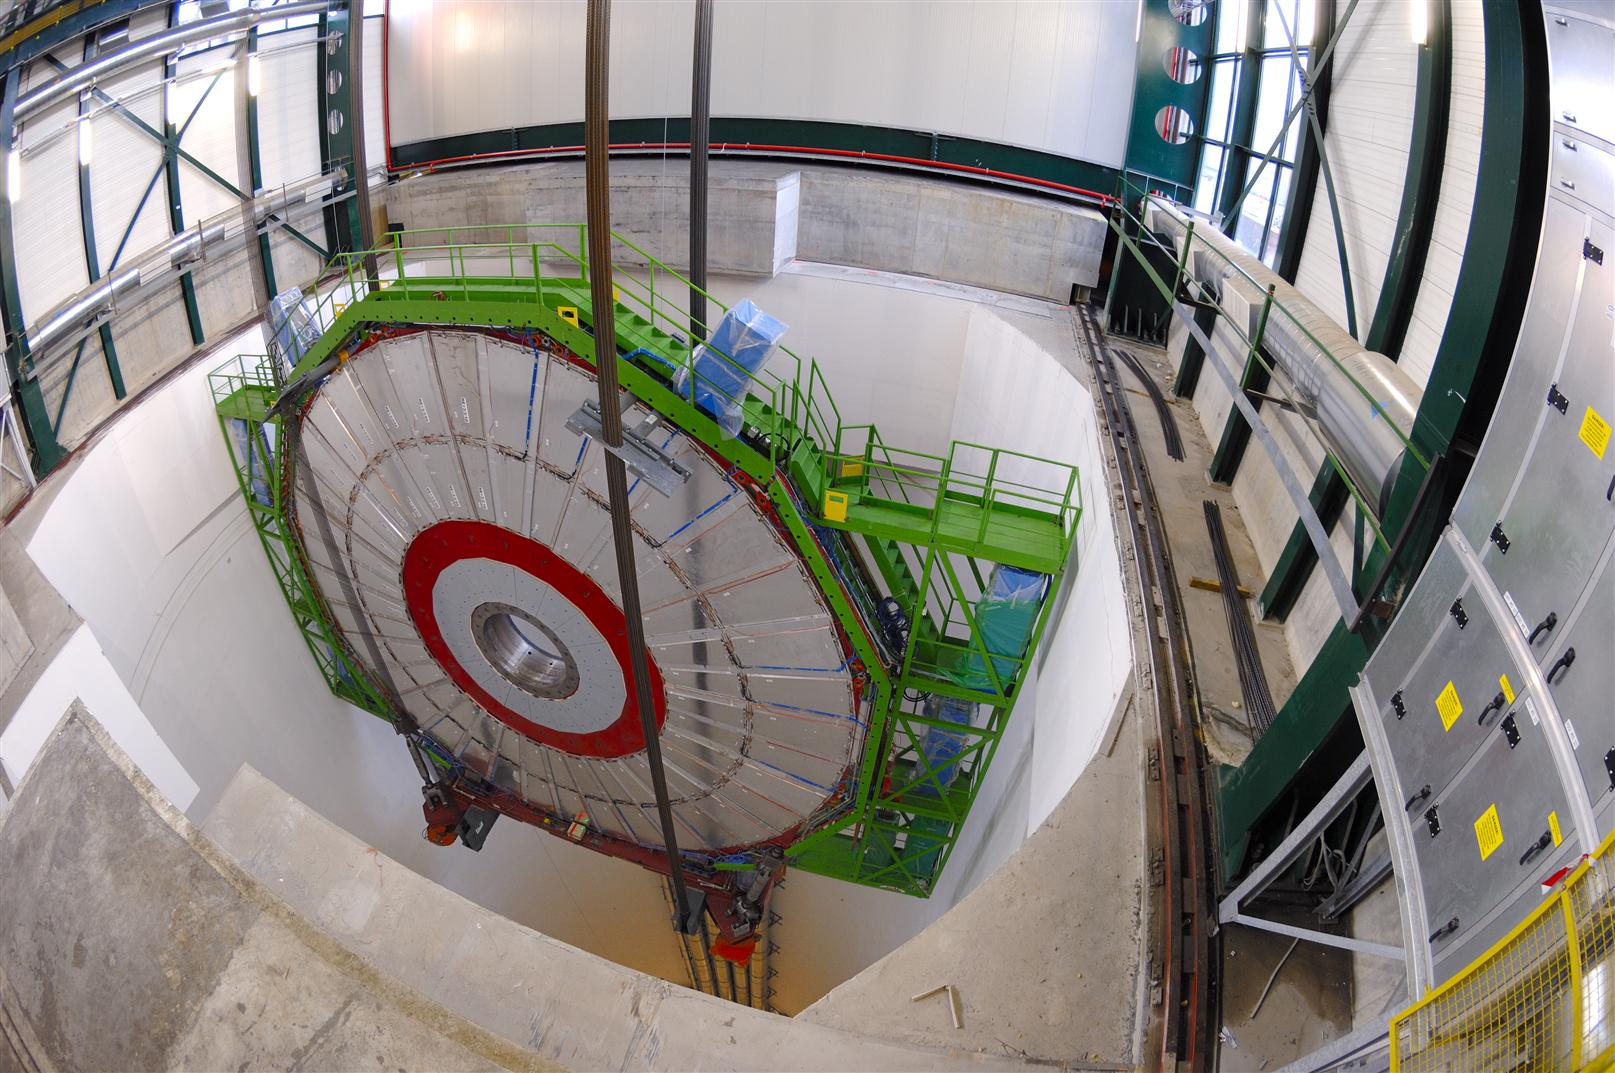
\includegraphics[width=\marginparwidth]{CMS/slice.jpg}
	\captionof{figure}{Descente d'une tranche de CMS.}
	\label{slice}
}
Chaque tranche à ensuite été descendue dans la caverne et assemblée à 100 m sous terre (cf.fig\ref{slice}).
CMS est une détecteur cylindrique de 24m de long et de 14.6 m de diamètre pour une masse de plus de 16000 tonnes (cf.fig\ref{cmsexploded}). Il est composé d'une succession de sous-détecteurs concentriques.

\begin{sidewaysfigure}
	\centering
	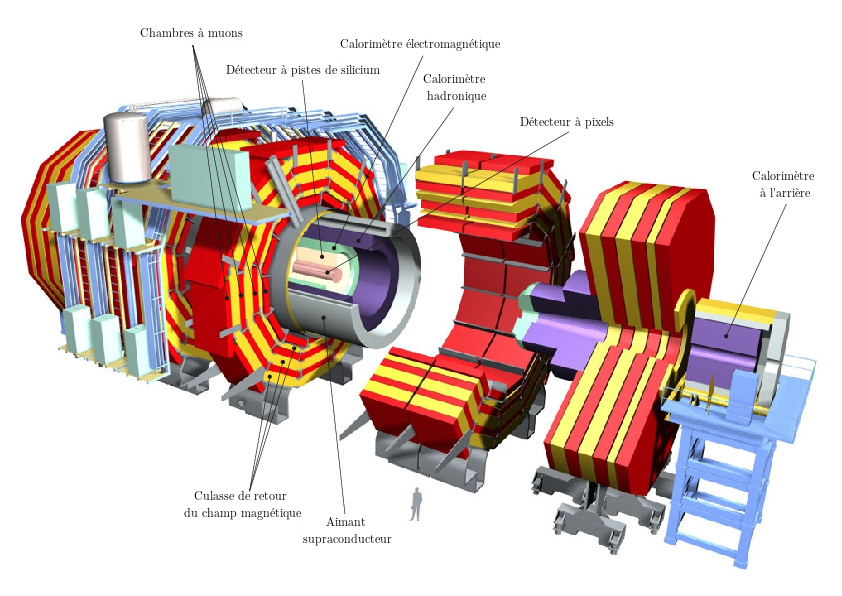
\includegraphics[width=0.80\textwidth]{CMS/cms.png}
	\caption{\label{cmsexploded}Vue éclatée du détecteur CMS.}
\end{sidewaysfigure}
\newpage
En partant du centre vers l'extérieur :
\begin{itemize}[label=$\bullet$]
	\item \textbf{Le trajectographe : } C'est le sous-détecteur le plus proche du point d'intéraction. Il permet de reconstruire la trajectoires des particules chargées.
	 \item \textbf{Le calorimètre électromagnétique (ECAL\footnote{Pour Electromagnetic CALorimeter.})}: Il permet de mesurer l'énergie des photons et des électrons.
	 \item \textbf{Le calorimètre hadronique (HCAL\footnote{Pour Hadronic CALorimeter})}: Il permet de mesurer l'énergie des hadrons.
	 \item \textbf{L'aimant supra-conducteur : } Il produit un champ de 3.8T et permet de courber la trajectoire des particules chargées.
	 \item \textbf{Les chambres à muons : } Elles permettent d'identifier, reconstruire la trajectoire et mesurer l'énergie des muons. 
\end{itemize}
Chaque composant de CMS fera l'objet d'une description plus détaillée dans les paragraphes suivants.

\section{Les sous detecteurs de CMS}
\subsection{Le trajectographe}
Le trajectographe de CMS (cf.fig\ref{trajectographe}) est le détecteur le plus proche du faisceau et du point de collision. Le trajectographe est composé de deux sous-détecteurs : le détecteur à pixels et le trajectographe à micro-piste de silicium. Il a pour but de reconstruire les traces des particules chargées issues des collisions grâce à des suites d'impacts enregistrés par les couches du détecteur. La trace reconstruite permet de déterminer la charge et l'impulsion de la particule associée. En effet, une particule de charge $q$ qui se déplace dans un champ magnétique subit une force donné par la formule de Lorentz. La trajectoire de la particule dans le cas d'un champ magnétique d'intensité $B$ est hélicoïdale, de rayon $R_{c}$. Il est ainsi possible dans déduire l'impulsion transverse :
\begin{equation}
p_{T}=qBR_{c}
\end{equation}
En prenant les positions selon r des hits, il est possible d'en déduire l'angle $\theta$, angle entre la trajectoire de la particule est le faisceau et donc de calculer l'impulsion totale:
\begin{equation}
p=\frac{p_{T}}{\sin\theta}
\end{equation}
\begin{figure}[ht!]
	\centering
	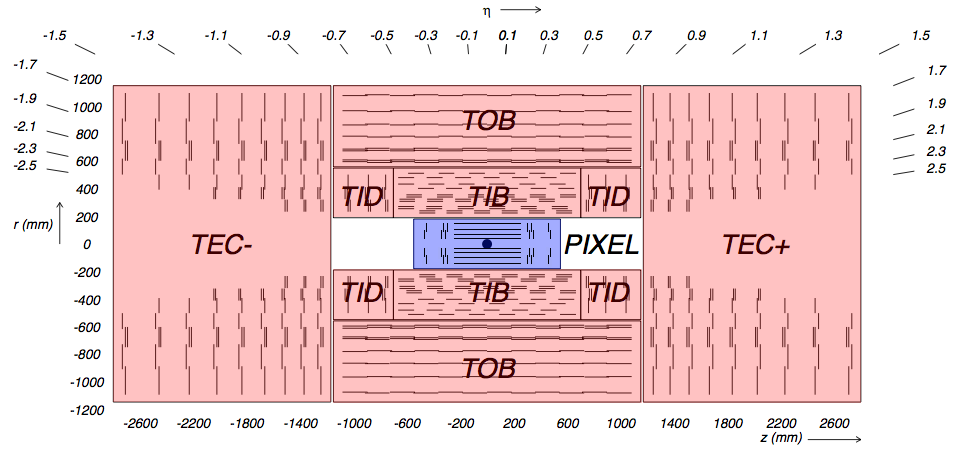
\includegraphics[width=0.65\textwidth]{CMS/tracker.png}
	\captionof{figure}{Schéma du trajectographe de CMS. Chaque trait représente un module du détecteur. Les lignes doubles correspondent à des modules mis dos à dos produisant des hits dit stéréo. Le détécteur à pistes est composé de quatre sous-détecteurs : Les tonneaux internes (TIB), les tonneaux externes (TOB), les disques interne (TID) et les bouchons (TEC).}
	\label{trajectographe}
\end{figure}

\subsubsection{Le détecteur à pixels}
Le détecteur à pixels de CMS a récemment été remplacé afin de garder une trajectographie performante à des luminosités au dessus de $2\times10^{34}cm^{-2}s^{-1}$ et avec un empilement de plus de $50$. Ce remplacement a eu lieu du 28 février au 7 mars 2017 durant l'arrêt technique hivernal prolongé (EYETS). Le nouveau détecteur à pixels se compose d'un tonneau constitué de quatre couches de détection (BPIX) à des distances du faisceau $r=3.0$cm, 6.8cm, 10.2cm et 16cm et d'une longueur de 548.8mm et de trois bouchons (FPIX) situé à $\pm$29.1cm,$\pm$39.6cm et $\pm$51.6cm pour une couverture radiale allant de 4.5 à 16.1cm . Une comparaison entre l'ancien détecteur à pixel et le nouveau est donné fig.\ref{pixel}.

	\begin{figure}[ht!]
	\subfloat[Vue oblique-transverse comparant les couche des tonneaux de l'ancien (gauche) et du nouveau détecteur]{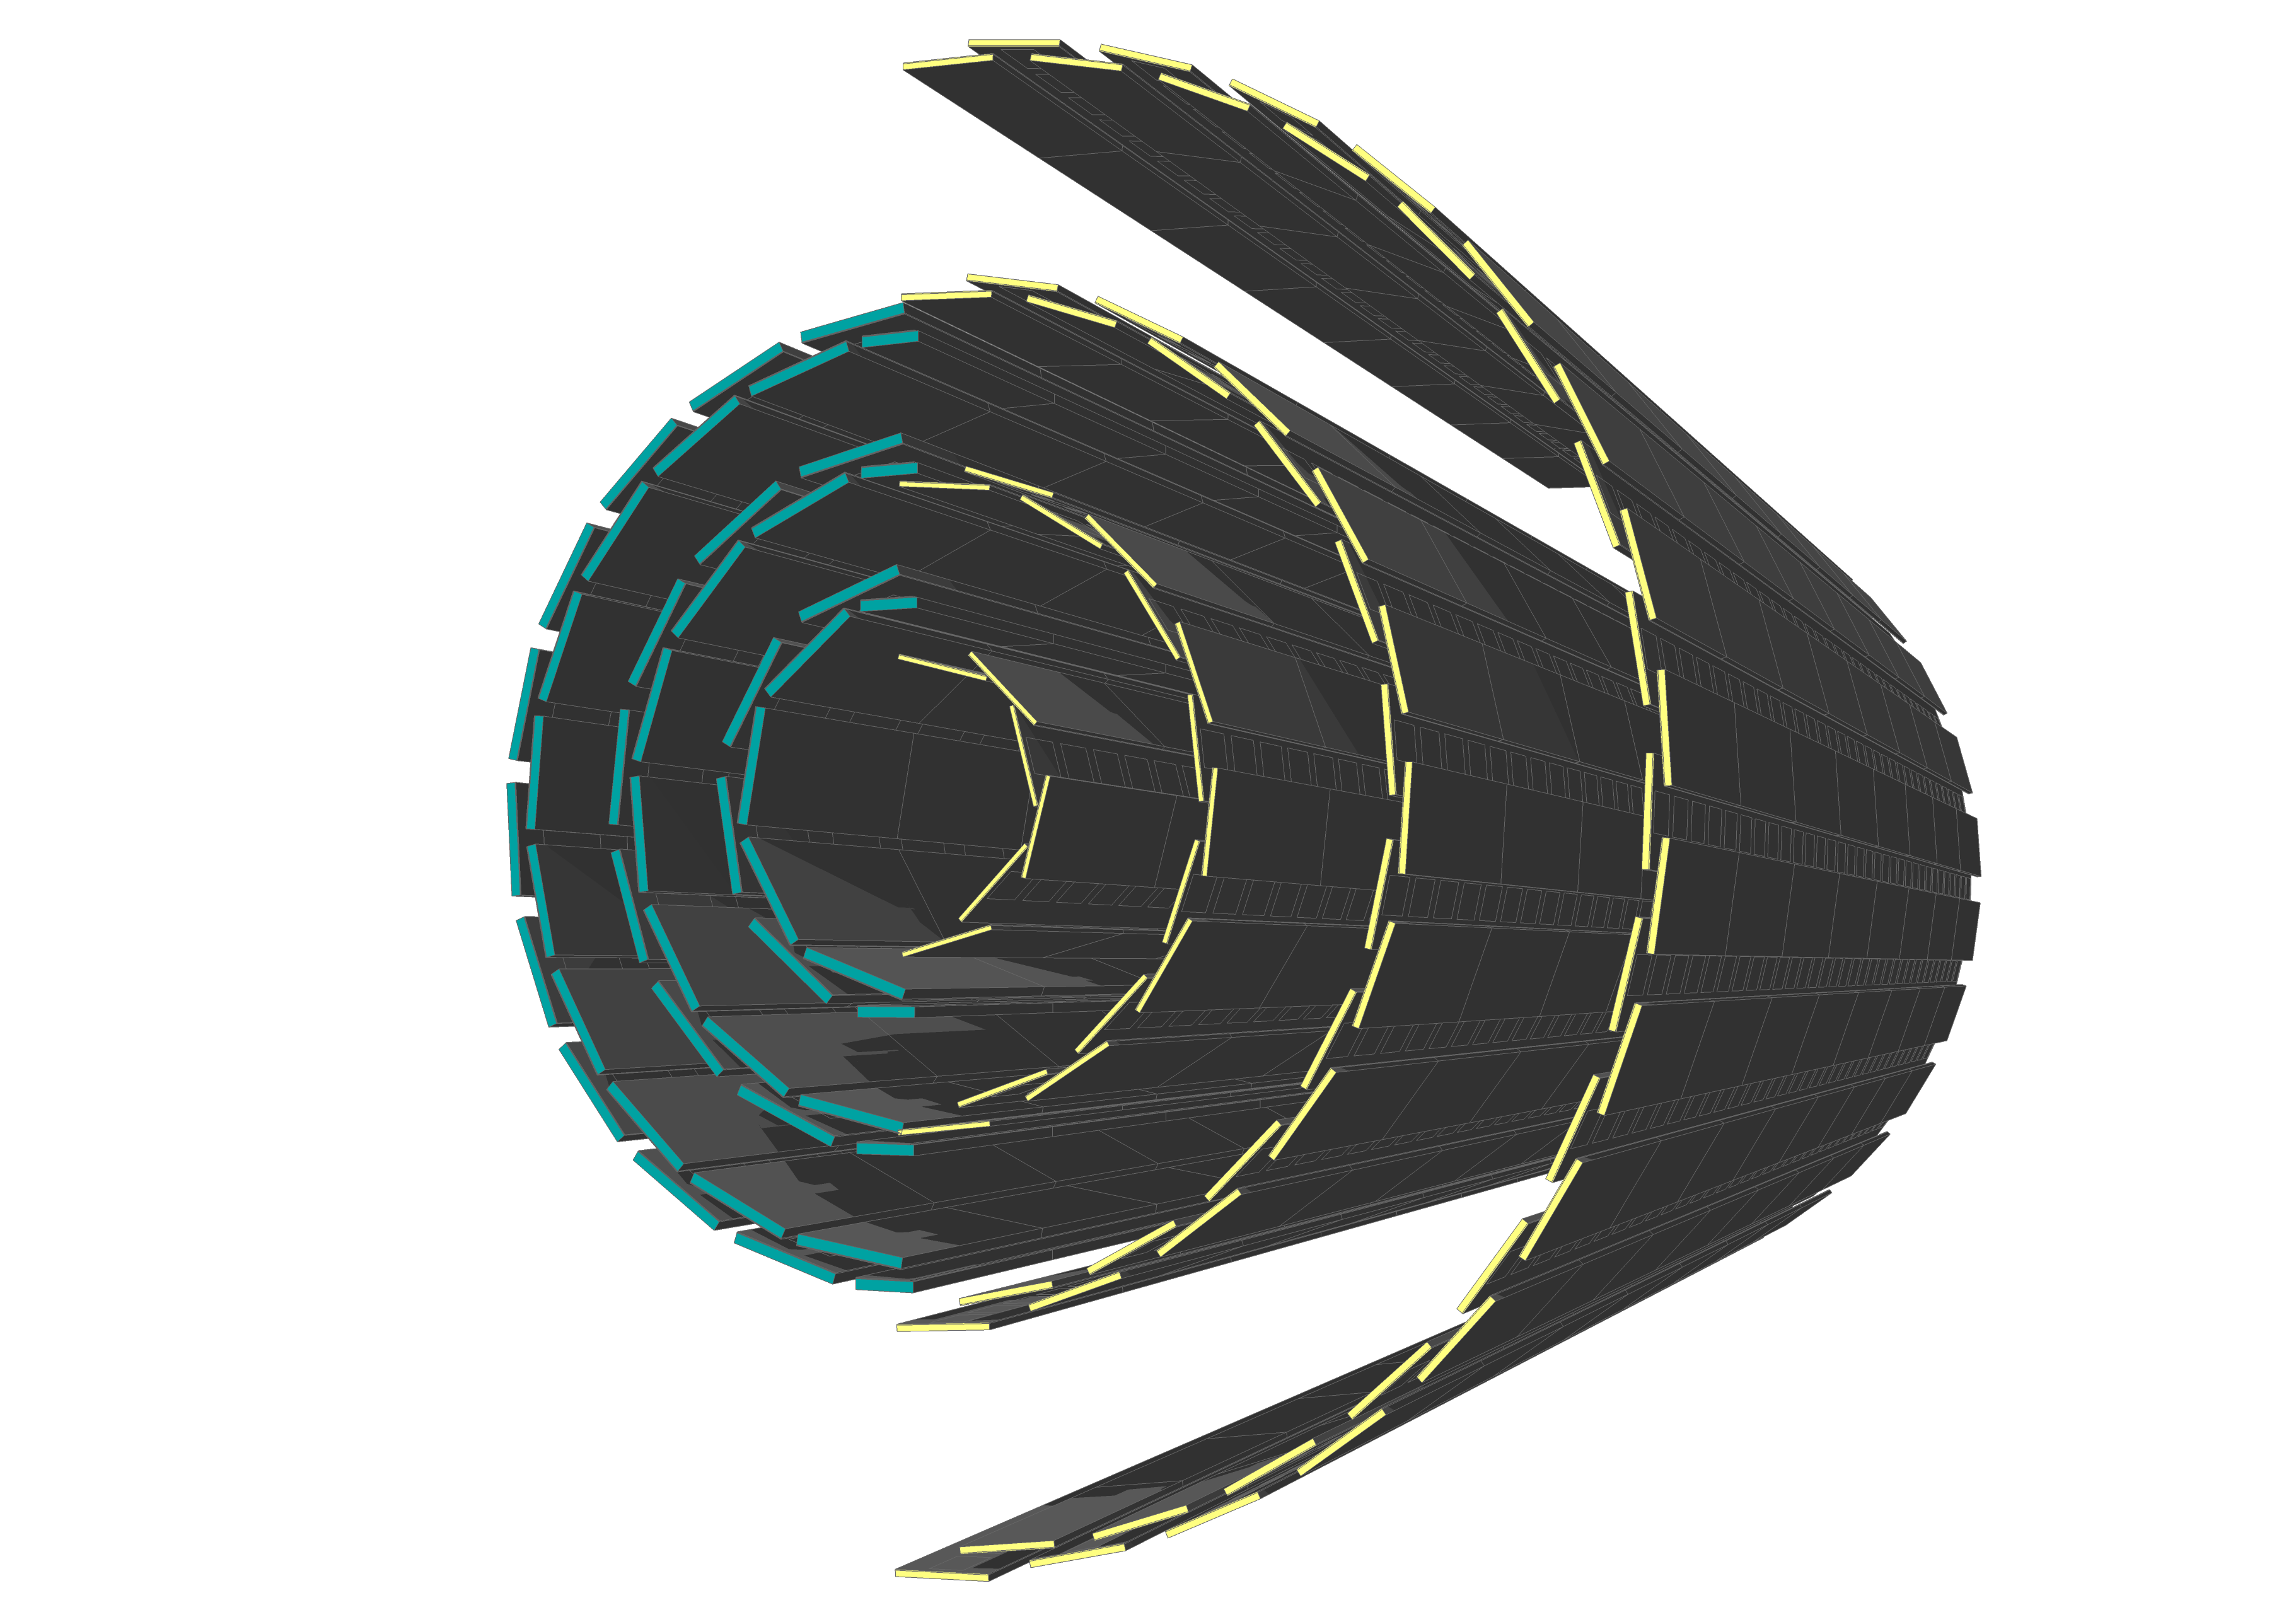
\includegraphics[width=.45\linewidth]{CMS/pixel.png}}
	\hfill
	\subfloat[Ancien détecteur à pixel (bas) et nouveaux (haut).]{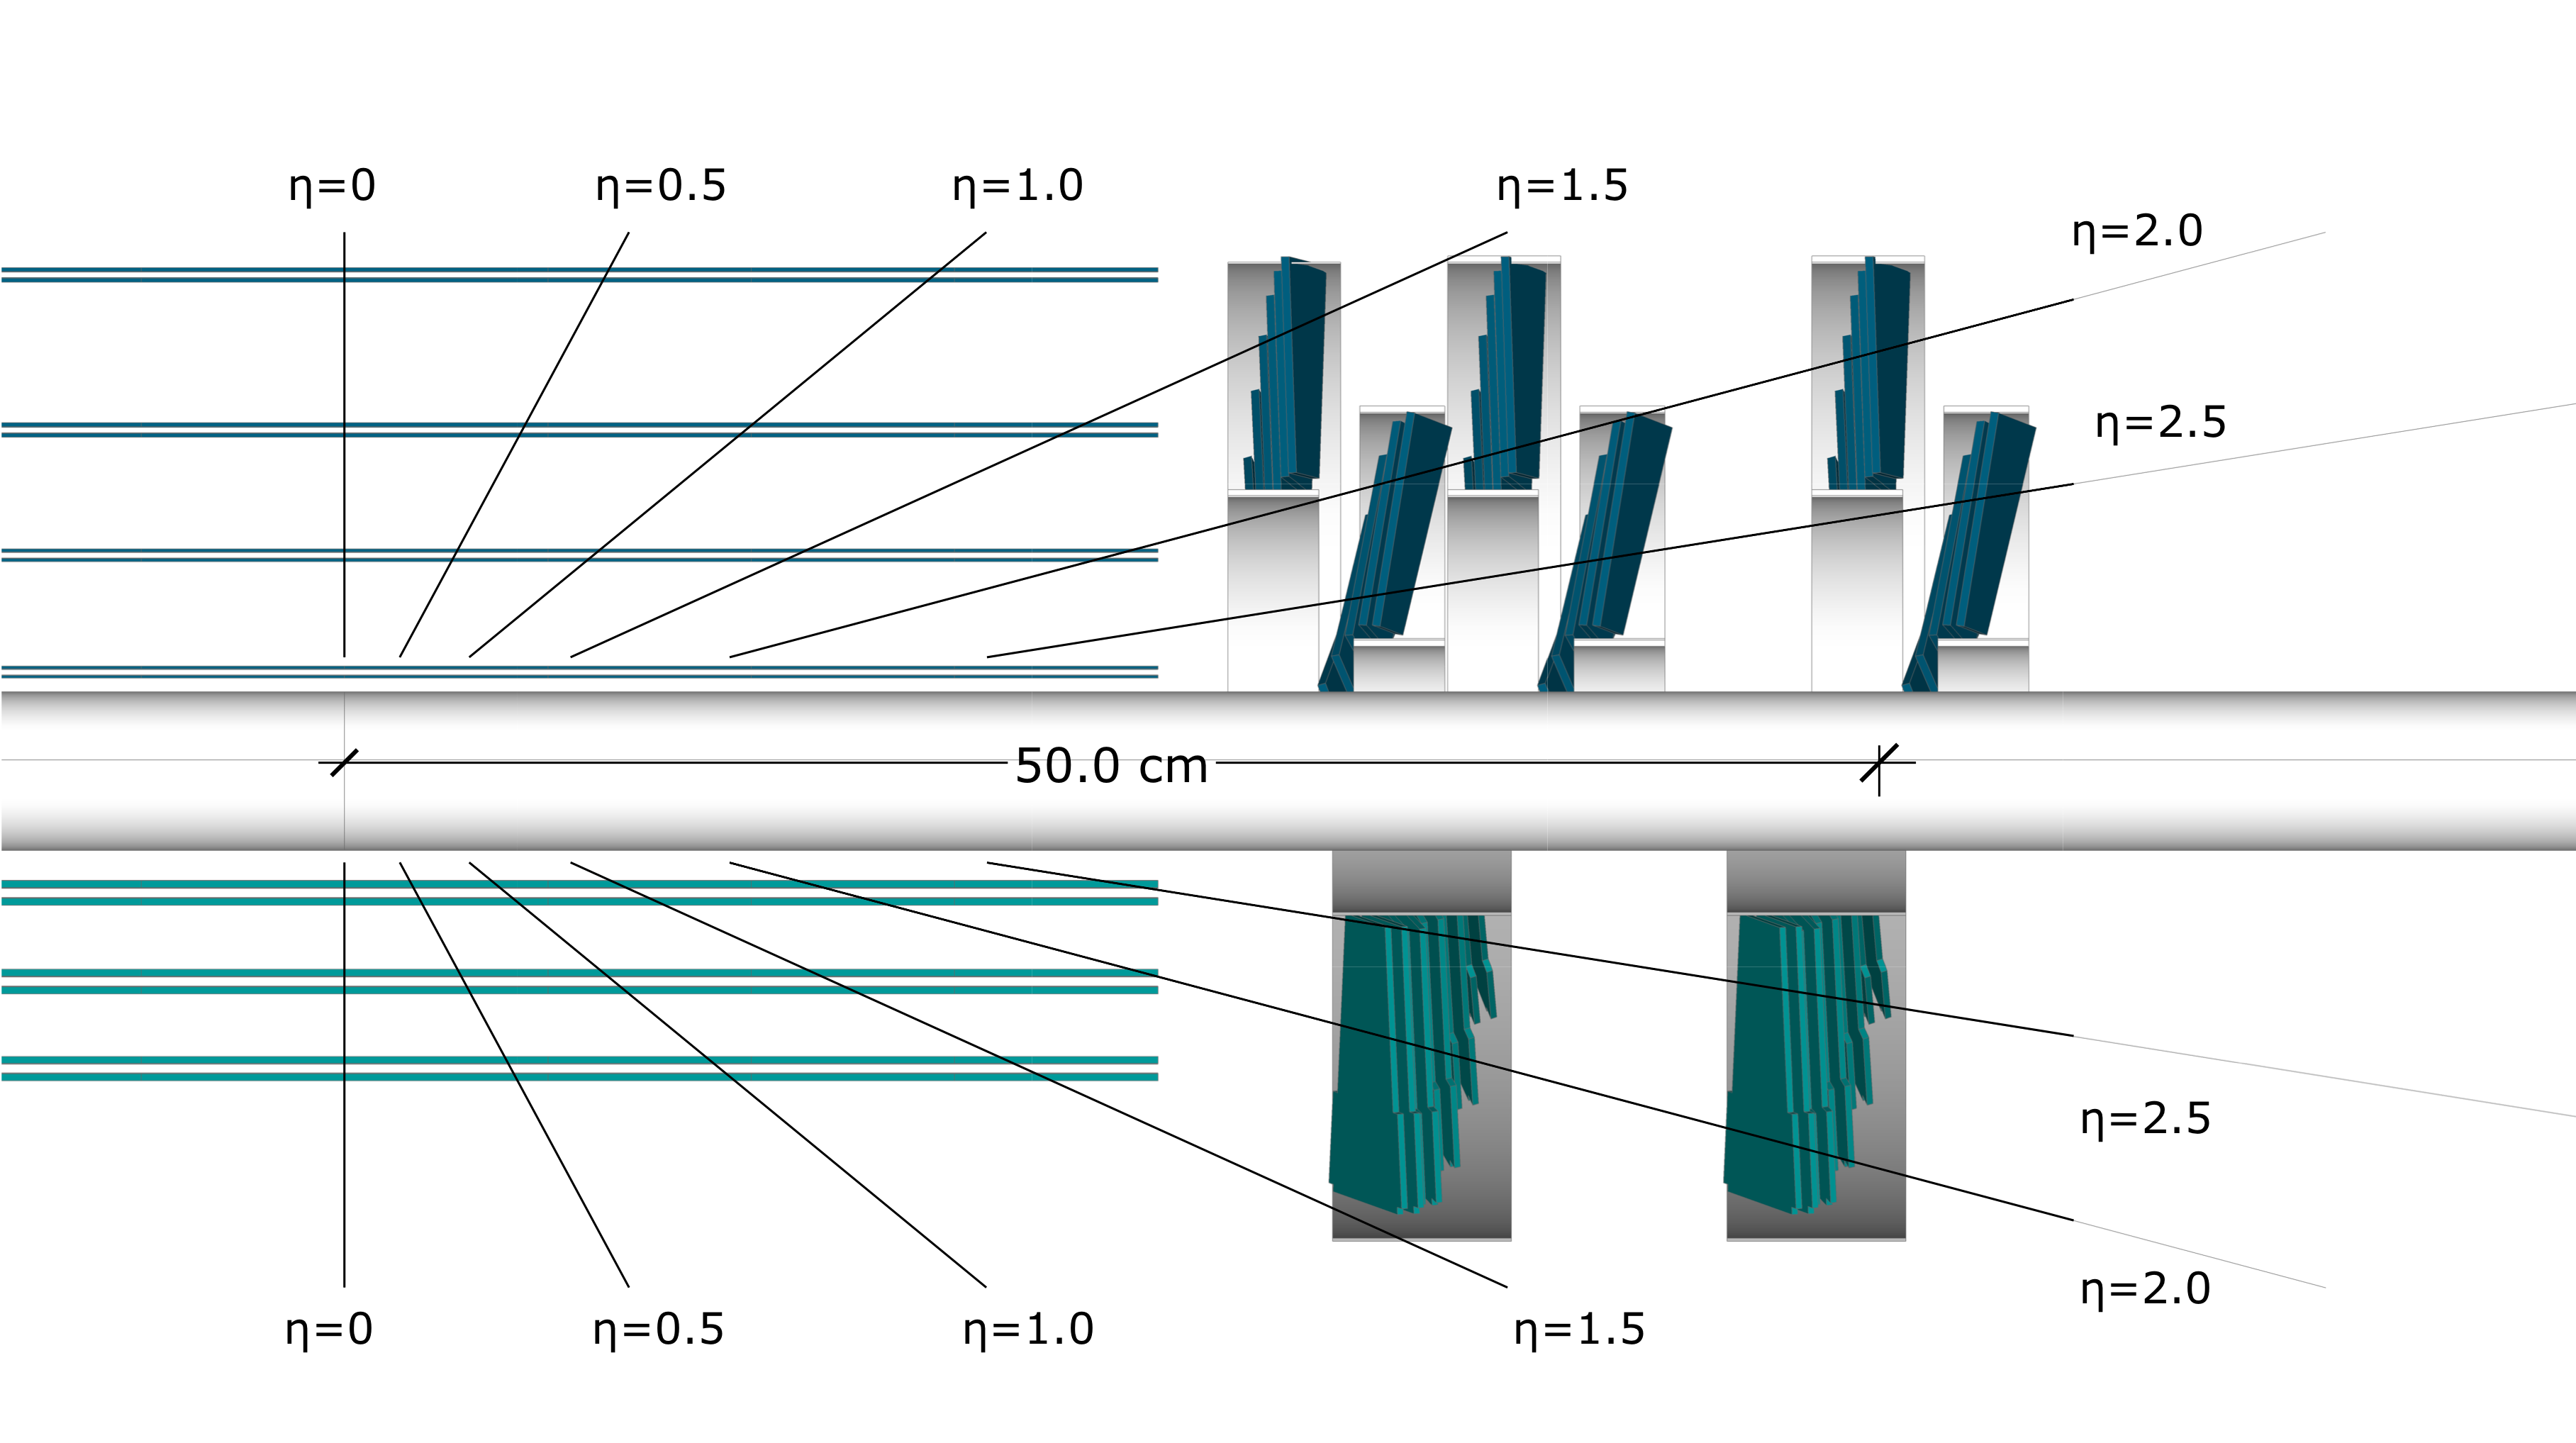
\includegraphics[width=.45\linewidth]{CMS/pixel2.png}}
	\caption{Comparaison entre le nouveau et l'ancien trajectographe à pixels.}
	\label{pixel}
\end{figure}

L'ajout d'une quatrième couche de détection dans le barrel assure une redondance lors de la reconnaissance de motifs et permet de réduire le taux d'erreur lors d'empilement importants. Il assure également une sécurité au cas où la couche la plus proche du point d'interaction viendrait à se détériorer plus vite que prévu. Cependant, elle augmente le budget matériel du détecteur, il a donc été nécessaire de repenser le support et les services afin d'être plus léger. Un nouveau système de refroidissement au $CO2$ ainsi que la déplacement des système passif (connectique , plaques d'électronique) hors du volume de trajectographie à également été effectué (cf.fig\ref{pixel2}).

\begin{figure}[ht!]
	\centering
	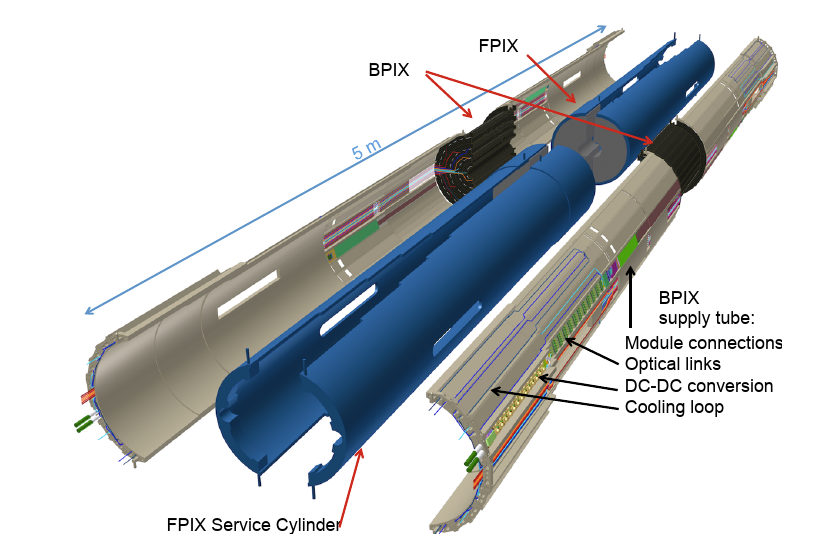
\includegraphics[width=0.80\textwidth]{CMS/pixel3.png}
	\captionof{figure}{Vue explosée du nouveau détecteur à pixels. La figure montre les positions des différentes partitions FPIX et BPIX ainsi que leur cylindres contenant leur service respectifs. Les services nécessaires au détecteur (connectiques, fibre optique, convertisseur DC-DC sont situés à haut $\eta$, hors du volume de trajectographie.)}
	\label{pixel2}
\end{figure}

Ce détecteur contient plus de 97 millions de pixels (79 pour les BPIX et 18 pour les FPIX) mesurant $100\times150\mu m$ de section et $250\mu m$ d'épaisseur. Ces pixels sont regroupés en modules (1184 pour BPIX et 672 pour FPIX) (cf.fig\ref{module}) de 66560 pixels  (8$\times$ 2 ROCs) d'une épaisseur de $75\mu m$ pour la première couche du BPIX et $250\mu m$ pour les reste du BPIX et FPIX.

	\begin{figure}[ht!]
	\centering
	\subfloat[Module pour les couches 2 à 4 des BPIX et des FPIX (gauche) et de la couche 1 de BPIX (droite)]{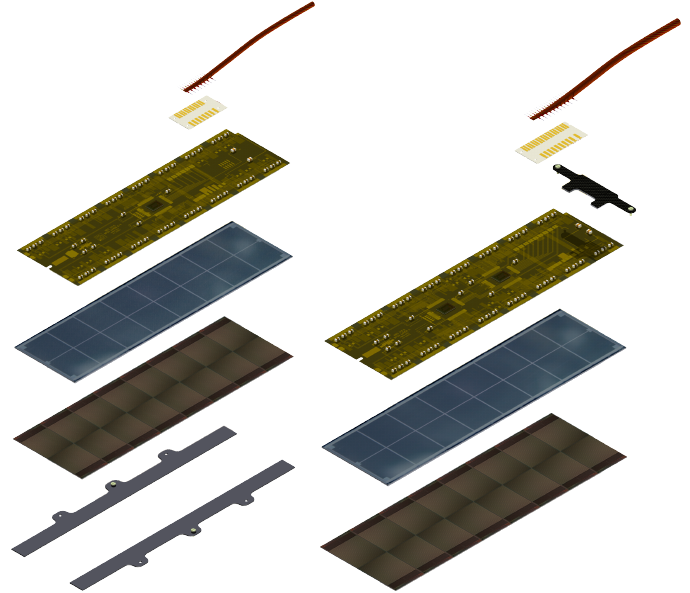
\includegraphics[width=.46\linewidth]{CMS/module.png}}
	\subfloat[Schéma de l'électronique de lecture d'un module]{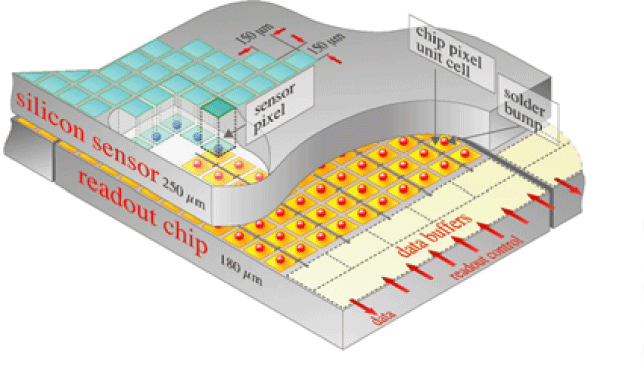
\includegraphics[width=.46\linewidth]{CMS/module2.png}}
	\caption{Modules de pixels.}
	\label{module}
\end{figure}
\subsubsection{Le détecteur à pistes}
Le détecteur à pistes mesure 5.5 m de long pour 2.4 m de diamètre pour une aire active de 198m2 et est le plus grand détecteur au silicium jamais construit. Il comporte en tout 15148 modules pour un total de 9.3 millions de pistes lues par 76000 puces électroniques. Il peut être décomposé en quatre sous-détecteurs :

\begin{itemize}[label=$\bullet$]
\item \textbf{Le tonneau interne} Le tonneau interne (TIB) (cf.fig\ref{TIB}) pour  \textit{Tracker Inner Barrel} est composé 2724 modules répartis en quatre couches. Chaque couche se compose de pistes de silicium d'une épaisseur de $320 \mu m$ avec un pas de $80 \mu m$ pour les deux premières couches et de $120\mu m$ pour deux dernières. Elles sont orientées parallèlement au faisceau. Les deux premières couches sont composées de modules dits "stéréos" qui sont la juxtaposition de deux modules collés l'un l'autre avec un angle de $100mrad$ entre les deux. Ce qui permet d'avoir une résolution de $23$ à $34\mu m$ dans le plan transverse et de $230\mu m$ dans le plan longitudinal. Son rayon est compris entre 25 et 52 cm et sa longueur couvre le domaine $|z|<65cm$.

\item \textbf{Les disques internes} (TID) (cf.fig\ref{TID}) pour \textit{Tracker Inner Disk} sont composés de trois disques parallèles qui sont compris dans le domaine $75cm<|z|<110cm$. Chaque disque est composé de trois anneaux concentriques. Les 816 modules sont composés de strips d'une épaisseur de $320\mu m$ orientées radialement pour un pas compris entre $81\mu m$ et $158\mu m$. Comme pour le TIB, les deux premiers modules sont "stéréos".
\marginpar
{
	\centering
	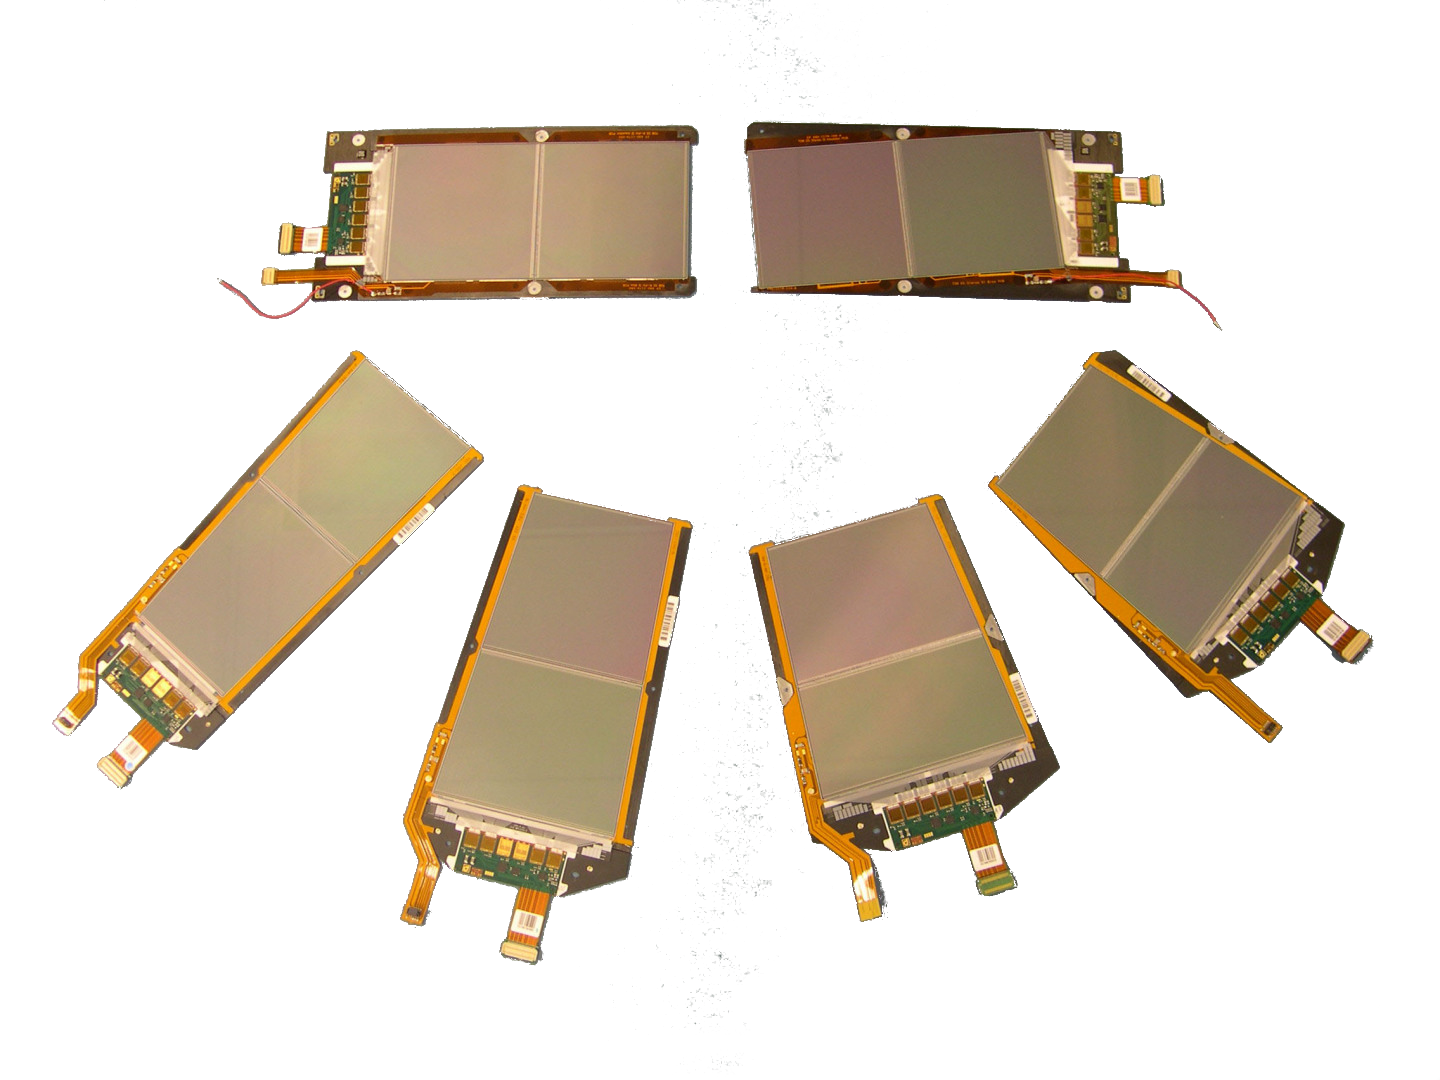
\includegraphics[width=\marginparwidth]{CMS/TOB_TEC.png}
	\captionof{figure}{Différents modules utilisés pour la construction du TOB et du TEC.}
	\label{TOB_TEC}
}
\item \textbf{Le tonneau externe } (TOB) (cf.fig\ref{TOB})pour \textit{Tracker Outer Barrel} entoure les TIB et TID pour couvrir un espace entre 60 et 100cm en rayon et $|z|<110cm$. Il est composé de 5208 modules (cf.fig\ref{TOB_TEC}) de pistes orientées parallèlement au faisceau et de pas compris entre 122 et 183 $\mu m$. Ces modules sont répartis en six couches dont les deux dernieres sont "stéréos". L'épaisseur de ces modules est de $500\mu m$.   

\item \textbf{Les bouchons }(TEC) (cf.fig\ref{TEC}) pour \textit{Tracker End-Cap} sont composés de neuf disques chacun, composée de 4 à 7 anneaux concentriques. Ils couvrent 25-110 cm en rayons et 120-275 cm en $|z|$. Les deux premiers disques ainsi que le cinquième sont "stéréos". Les trois premiers anneaux sont composés de 1256 modules par bouchon (cf.fig\ref{TOB_TEC}) d'épaisseur 320$\mu m$ et de pas inter-pistes compris entre 81 et 158 $\mu m$. Les quatre anneaux suivant, sont composés de 1944 modules par bouchon (cf.fig\ref{TOB_TEC}), d'épaisseur $500\mu m$ de pas inter-strip 113-172 $\mu m$.
\end{itemize}

	\begin{figure}[ht!]
	\centering
	\subfloat[Le TIB.]{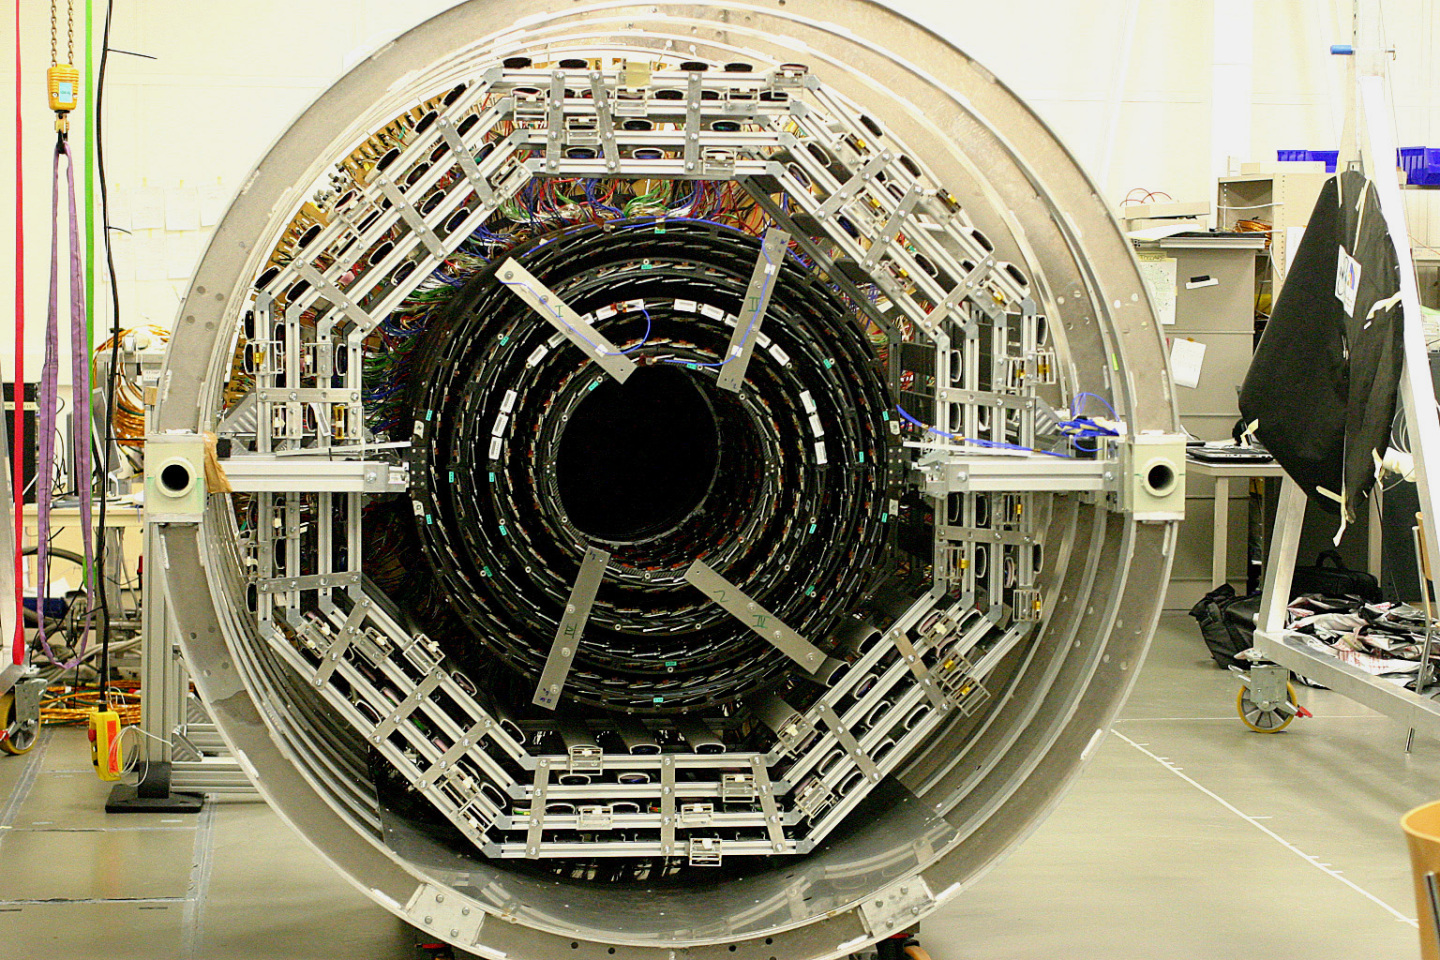
\includegraphics[width=.40\linewidth]{CMS/TIB.jpg}\label{TIB}}
	\subfloat[Un TID.]{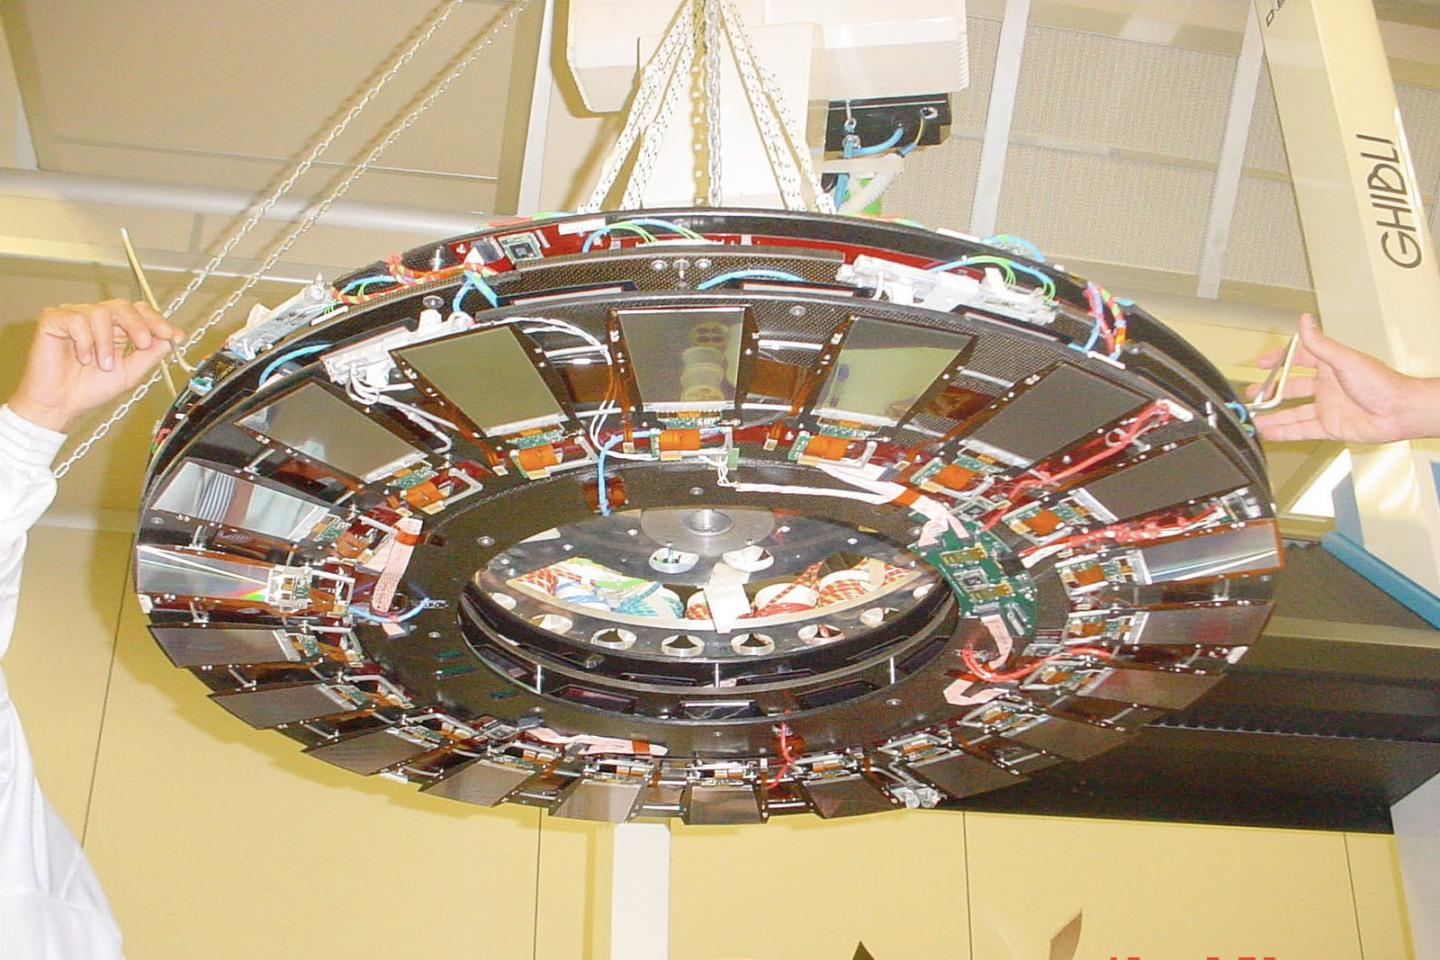
\includegraphics[width=.40\linewidth]{CMS/TID.jpg}\label{TID}}
	\\
	\subfloat[Le TOB.]{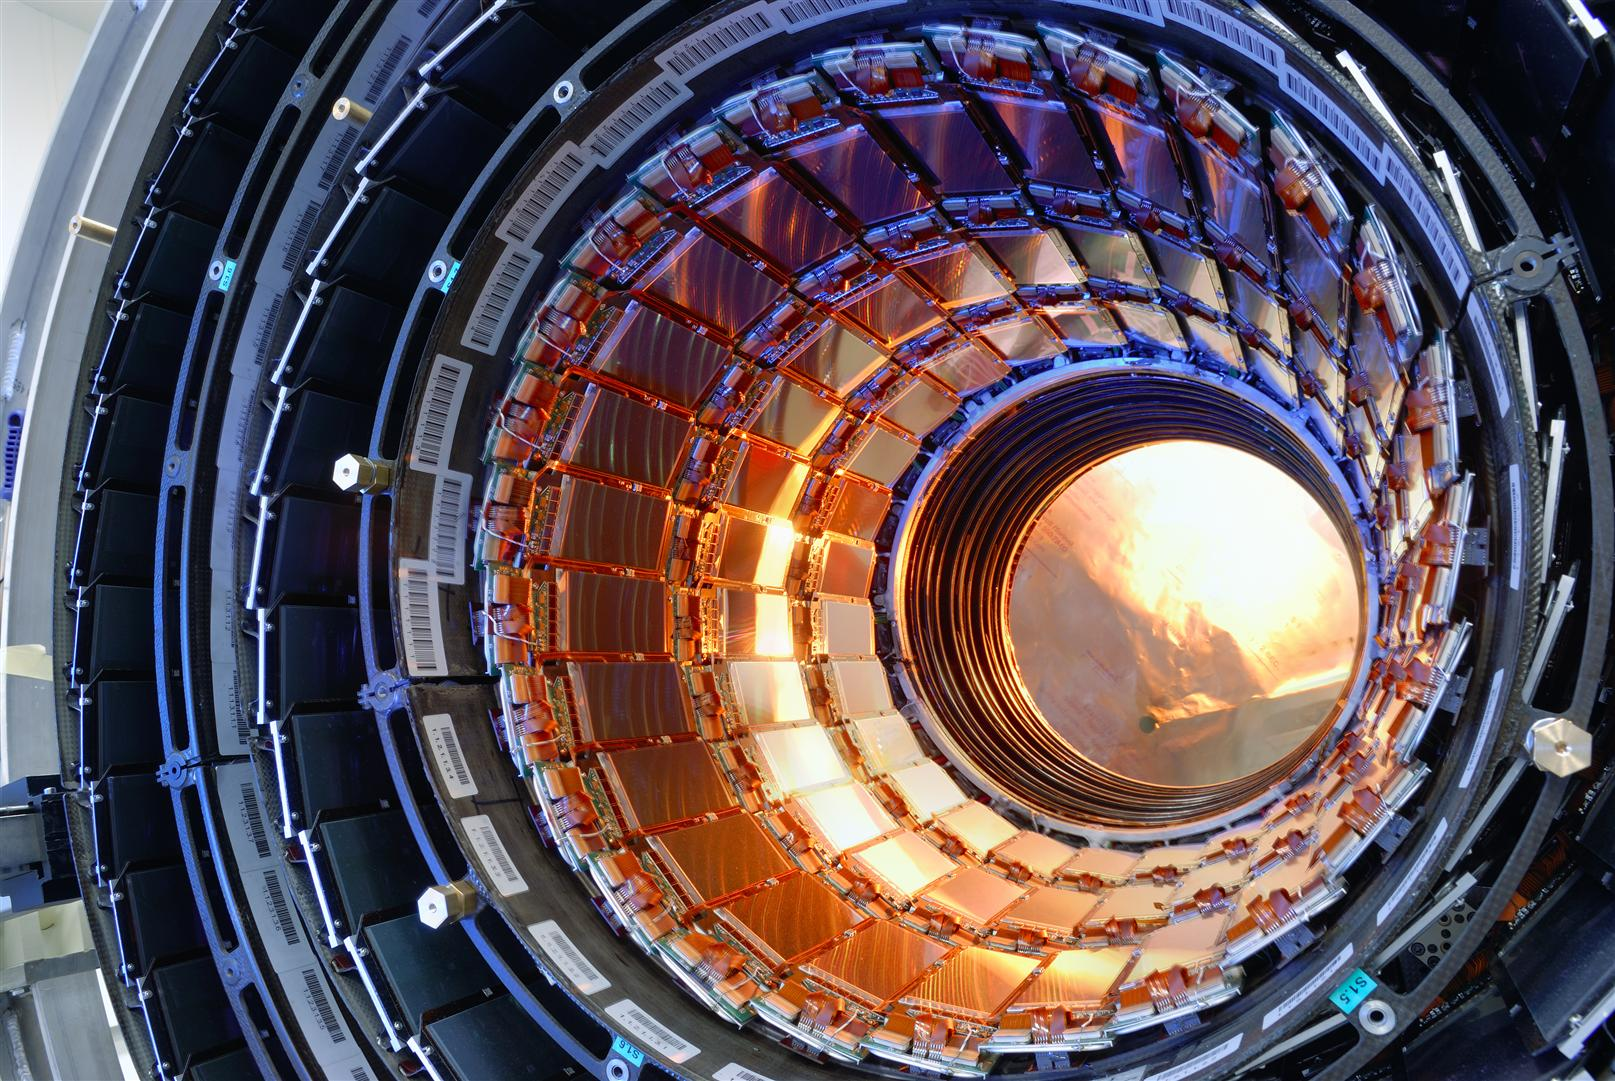
\includegraphics[width=.40\linewidth]{CMS/TOB.jpg}\label{TOB}}
	\subfloat[Un TEC.]{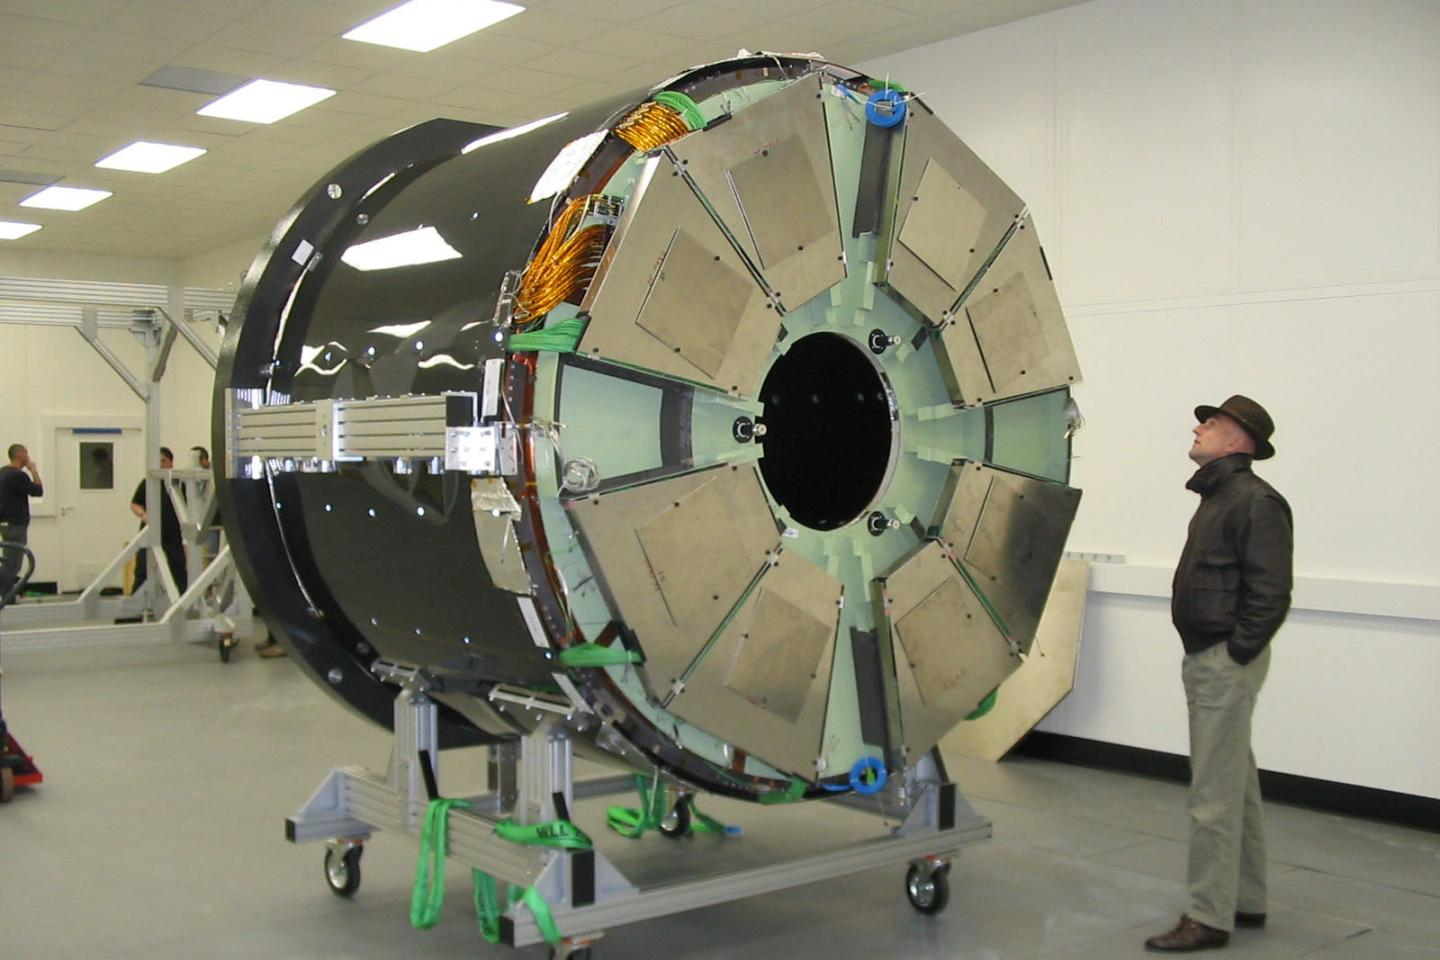
\includegraphics[width=.40\linewidth]{CMS/TEC.jpg}\label{TEC}}
	\caption{Photos des différents composants du détecteur à pistes}
\end{figure}

\newpage
\subsection{Le calorimètre électromagnétique}
Le calorimètre électromagnétique de CMS ou \textit{Electromagnetic CALorimeter} (ECAL), permet de mesurer l'énergie et la direction des particules réagissant principalement à l'interaction électromagnétique. Ce sont surtout les photons et les électrons qui seront détectés; ils perdent leur énergie par des processus radiatifs. La distance caractéristique est donnée par la longueur de radiation $X_{0}$, dépendante du matériau, définie comme le libre parcours moyen pour le processus de radiaction. Des photons de 100 GeV perdent à peu près toute leur énergie dans 20*$X_{0}$.
\begin{figure}[ht!]
	\centering
	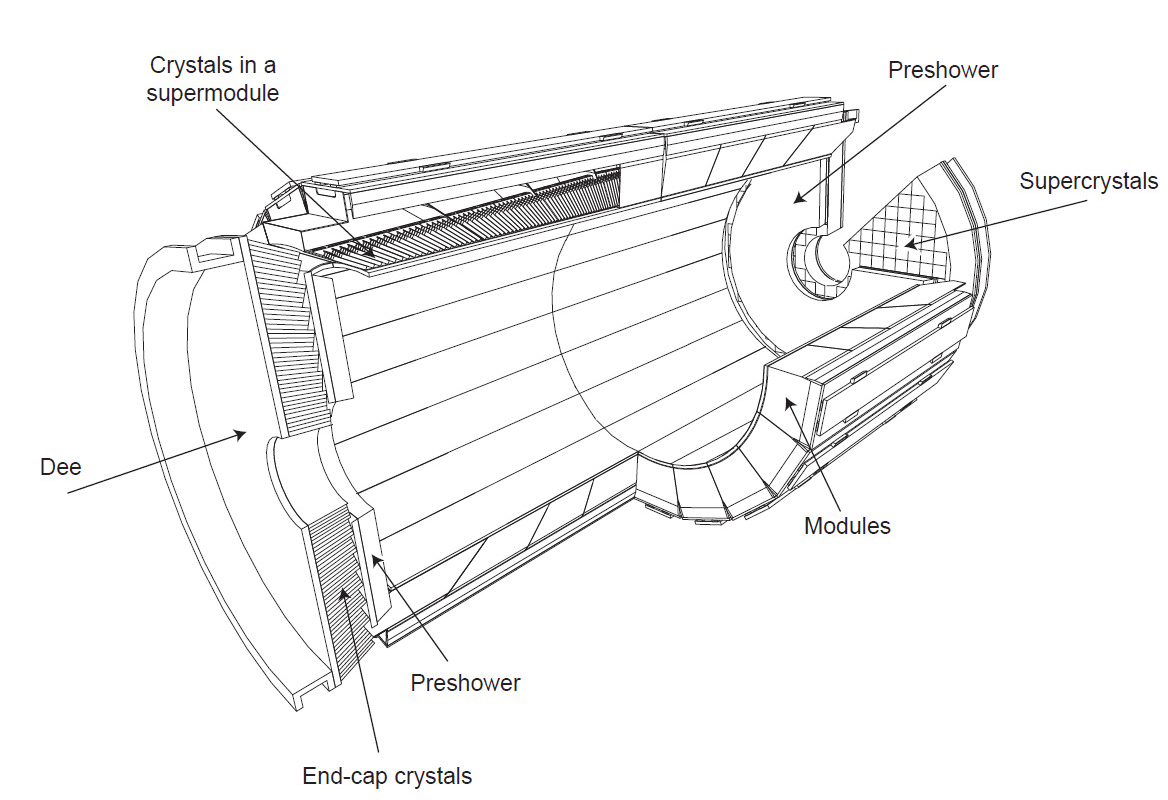
\includegraphics[width=0.90\textwidth]{CMS/ECAL.png}
	\captionof{figure}{Schéma du ECAL de CMS.}
	\label{ECAL}
\end{figure}

Le calorimètre électromagnétique est composé de 75848 cristaux (cf.fig\ref{crystaux}) de PbWO4 ($11 m^3$, 92 tonnes)et peut se décomposer en trois sous-structures (cf.fig\ref{ECAL}) :
\begin{itemize}[label=$\bullet$]
	\item \textbf{Le tonneau} ou EB (cf.fig\ref{EB}) pour \textit{Electromagnetic Barrel} contient 61200 cristaux de tungstate de plomb. Le tonneau est divisé en 36 supermodules couvrant chacun la moitié de la longueur du tonneau. Chaque super-module contient 1700 cristaux de 22*22 mm2 et de longueur 230 mm. Les cristaux sont arrangés de manière à former 170-$\eta$ anneaux contenant 360 cristaux chacun. Un cristal couvre environ 1$\degres$ en $\phi$. Le tonneau couvre une zone en pseudorapidité de $|\eta|<1.479$. Les photodiodes à avalanche (cf.fig\ref{APD}) (APD) sont utilisées pour détecter la scintillation.
	\marginpar
	{
		\centering
		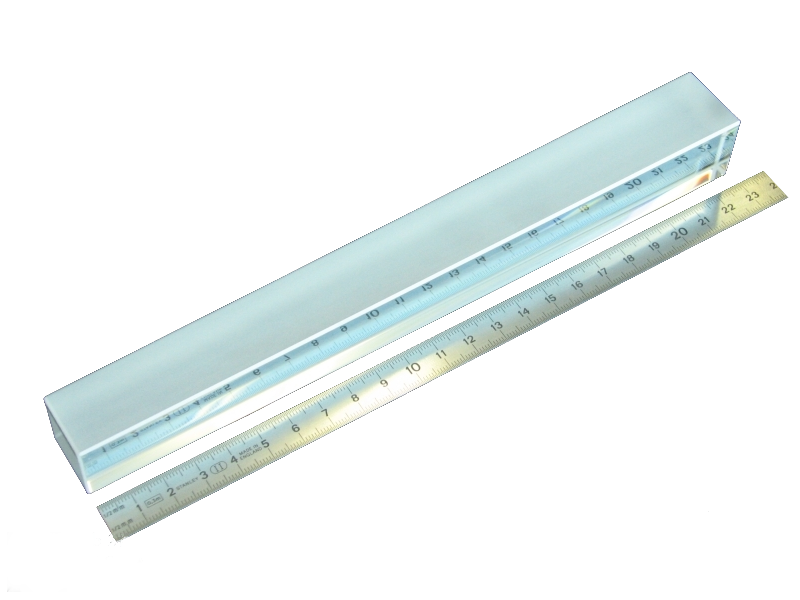
\includegraphics[width=\marginparwidth]{CMS/Crystaux.png}
		\captionof{figure}{Un cristal de PbWO4.}
		\label{crystaux}
	}
	
	\marginpar
	{
		\centering
		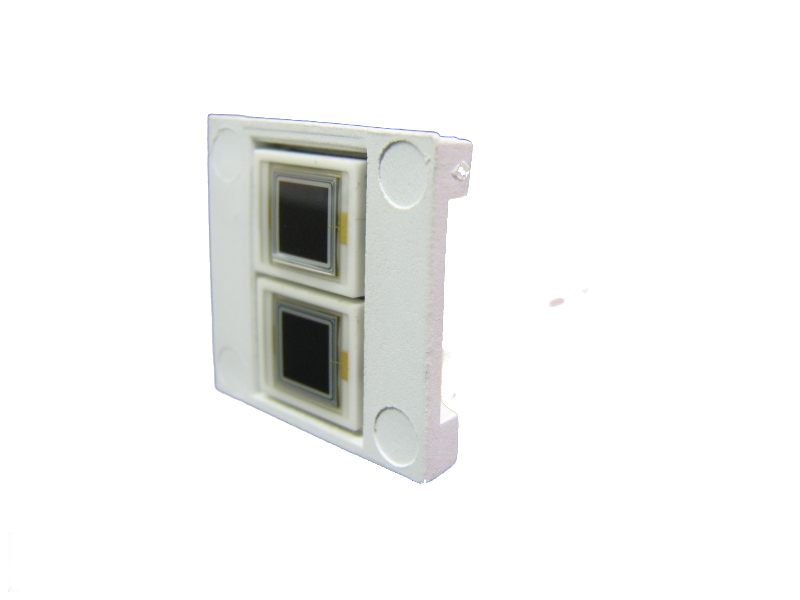
\includegraphics[width=\marginparwidth]{CMS/APD.png}
		\captionof{figure}{Un groupe de deux APD.}
		\label{APD}
	}
	\marginpar
	{
		\centering
		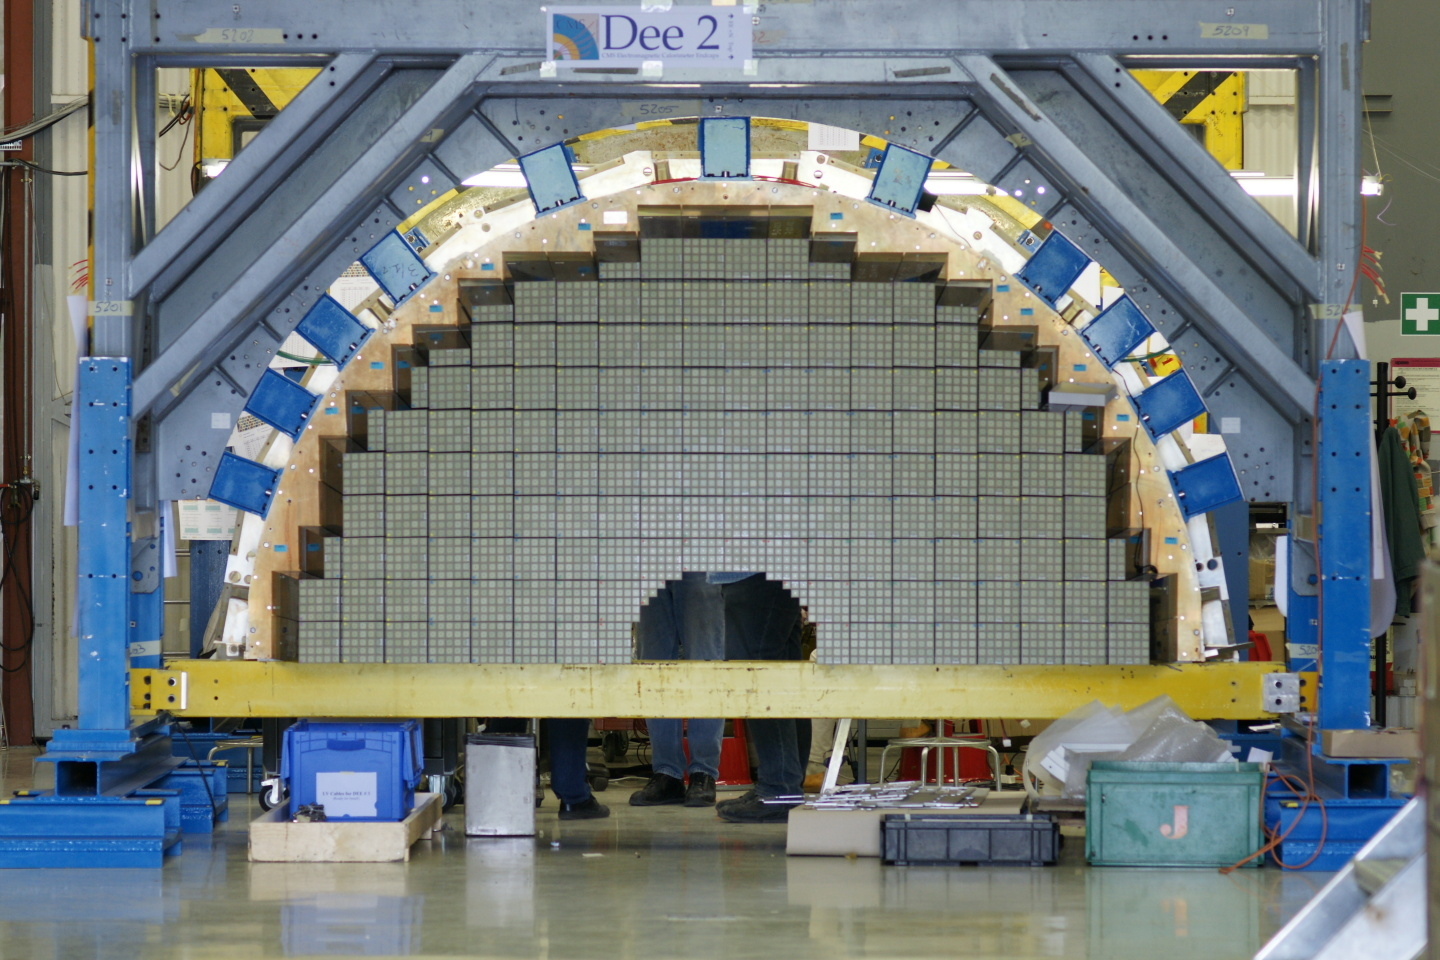
\includegraphics[width=\marginparwidth]{CMS/dee.jpg}
		\captionof{figure}{Un "Dee".}
		\label{DEE}
	}
	\marginpar
	{
		\centering
		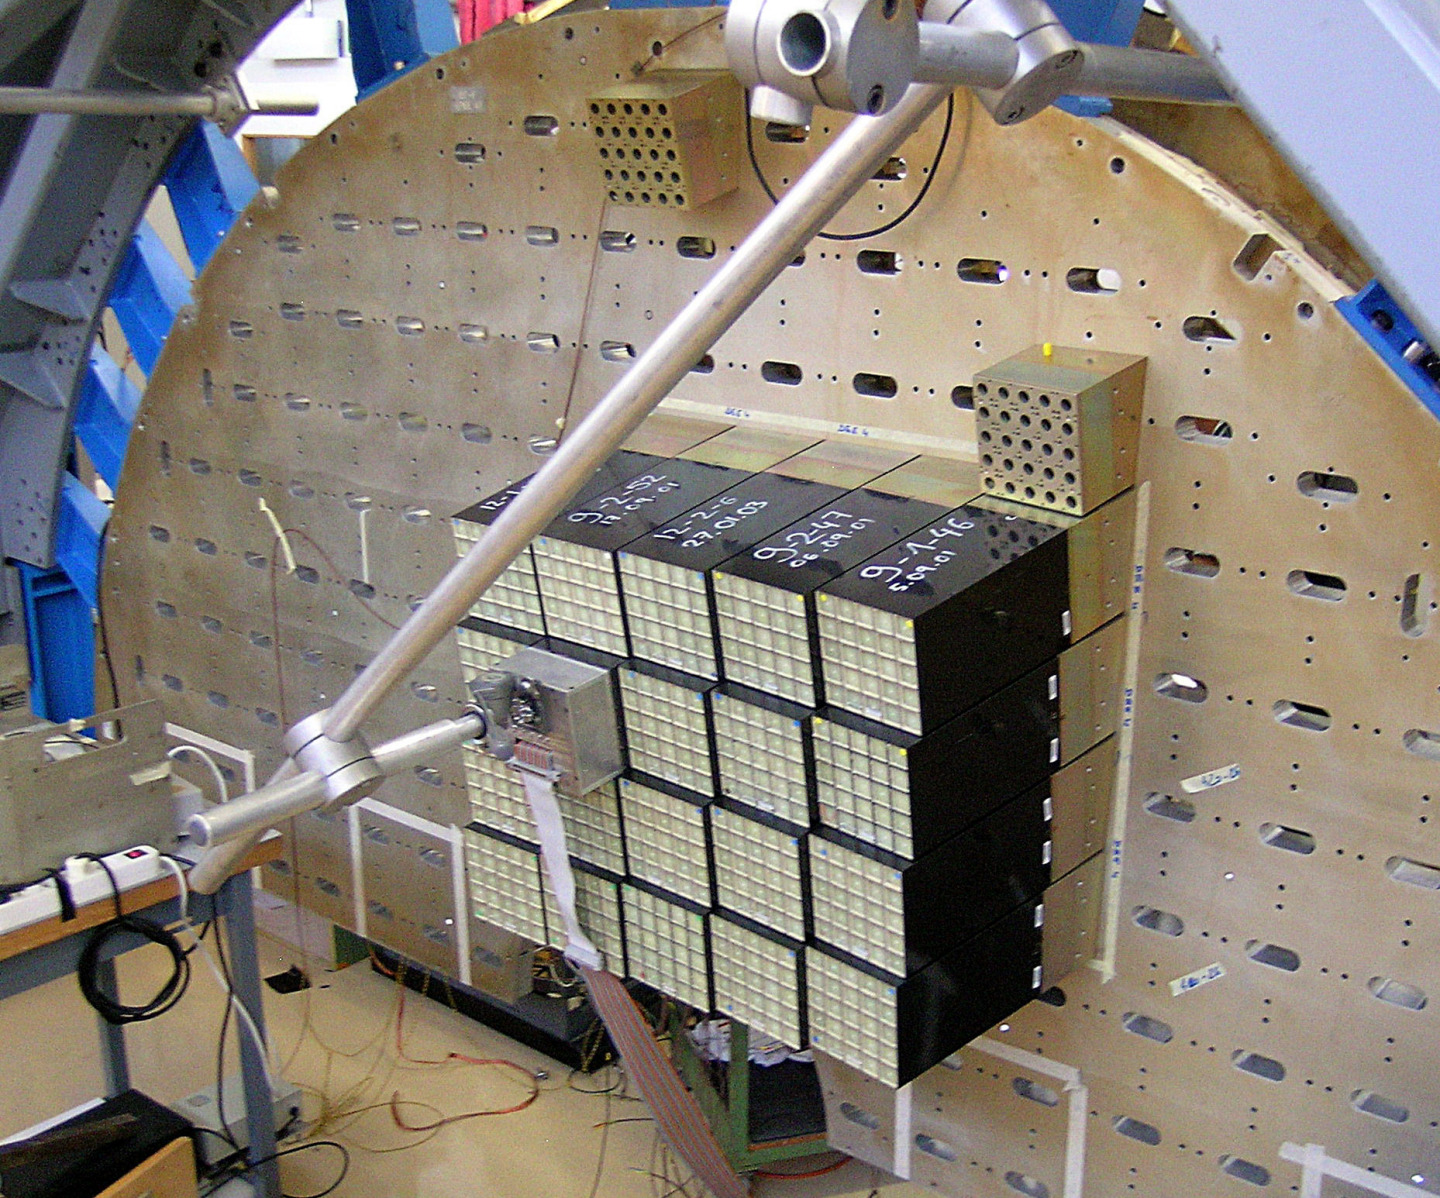
\includegraphics[width=\marginparwidth]{CMS/20SCs.jpg}
		\captionof{figure}{Montage de 20 Super-Cristaux sur un des Dee.}
		\label{SP}
	}
	\marginpar
	{
		\centering
		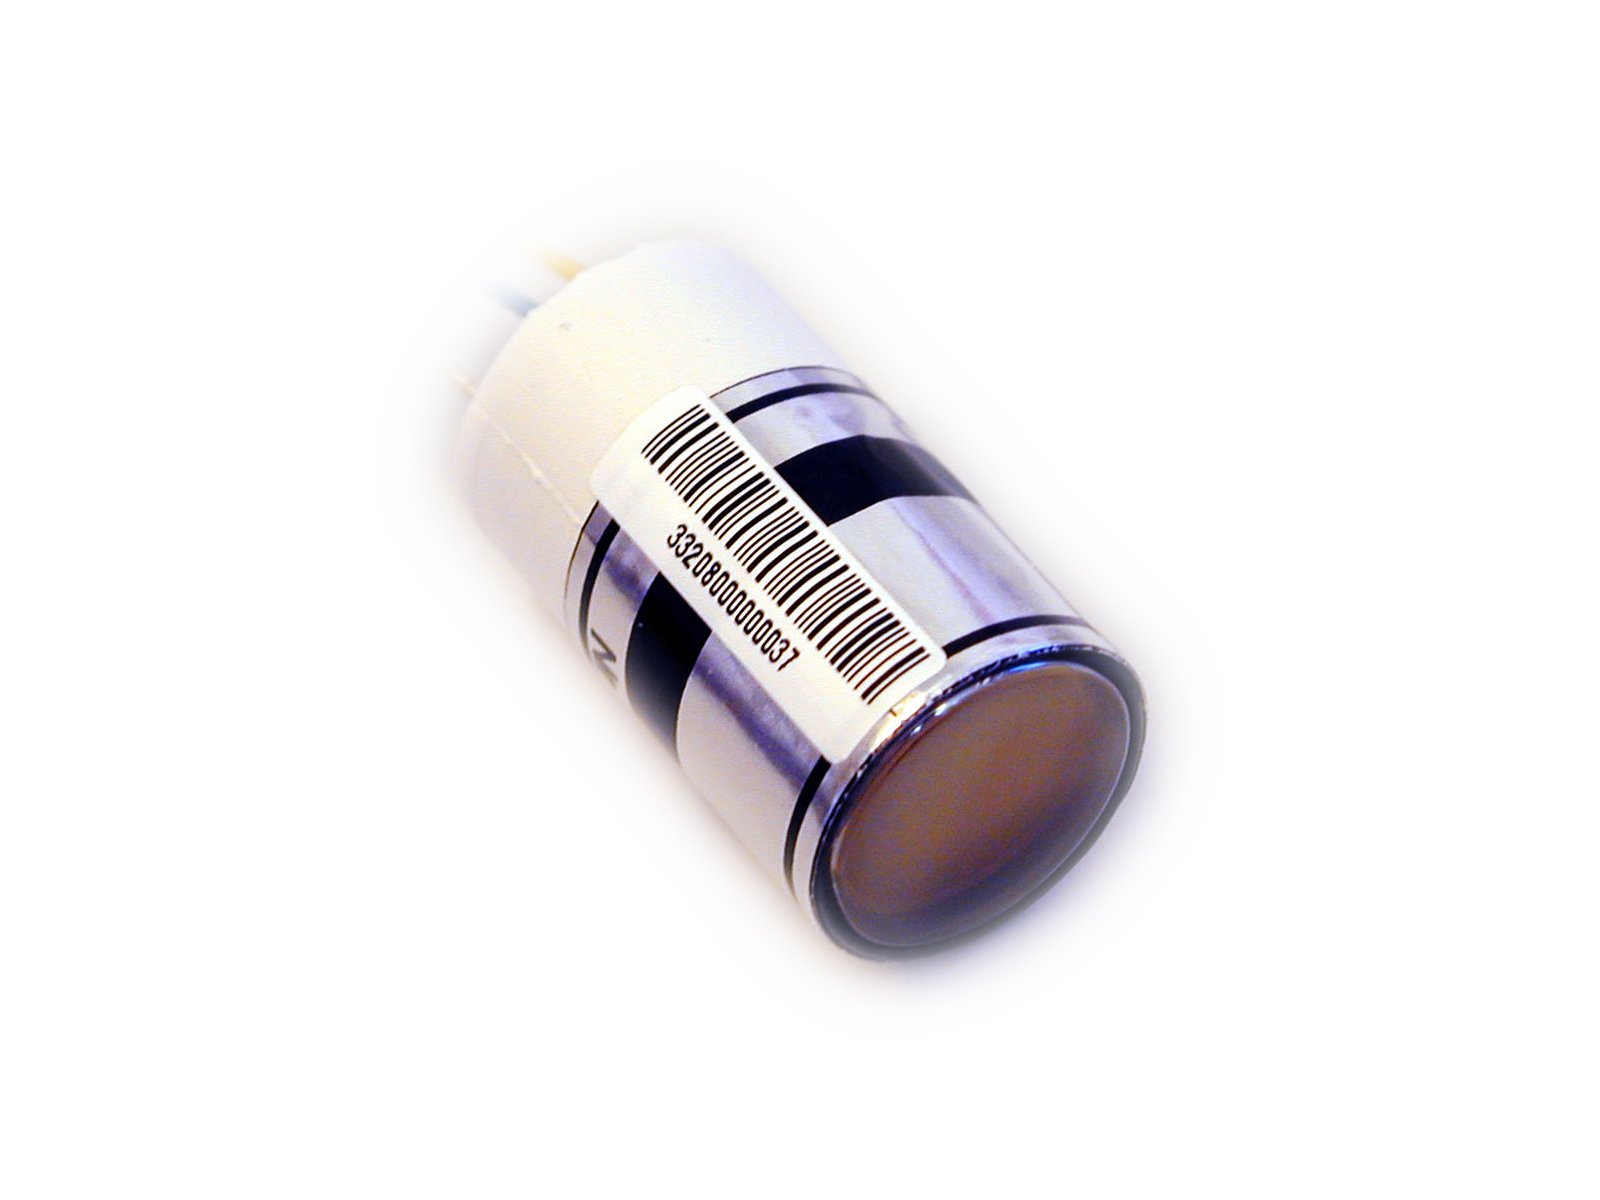
\includegraphics[width=\marginparwidth]{CMS/VPT.png}
		\captionof{figure}{Une VPT.}
		\label{VPT}
	}
	
	\item \textbf{Les bouchons} (EE) (cf.fig\ref{EE}) pour \textit{Electromagnetic End-cap} sont perpendiculaires au faisceau et ferment le EB. Ils sont situés à 315 cm du point d'interaction et couvrent une section en $\eta$ allant de 1.479 à 3. Chaque bouchon se décompose en deux demi-disques appelés "Dee" (cf.fig\ref{DEE}). Chaque Dee est constitué de 3662 cristaux de 2.86*2.86 cm et de longeur 220 mm regroupés en matrices de 5*5 qu'on appelle Super-Cristaux (cf.fig\ref{SP}). La scintillation est détecté par des phototriode à vide (VPT) (cf.fig\ref{VPT}). Les cristaux de PbWO4 ont une grande densité ($\rho=$8.28g.cm$^{-3}$), une longueur d'interaction $X_{0}$ assez courte de 0.89cm est un petit rayon de molière ($r_{M}$=2.2cm) ainsi qu'une grande vitesse de radiation (80\% dans 25 ns). 
	\item \textbf{L'initiateur de gerbe } (cf.fig\ref{PRESHOWER}), appellé \textit{Preshower} est placé entre le EB et le EE. Il consiste en deux couches de détecteurs de silicium de pas 1.9 mm intercalées entre deux couches en plomb (2$X_{0}$ devant et 1$X_{0}$ derrière la première couche de silicium). Il permet d'améliorer la précision de la mesure de la position de la gerbe électromagnétique et l discrimination $\gamma/\pi_{0}$. Il couvre une région comprise entre 1.653<$|\eta|$<2.6.
\end{itemize}
\begin{figure}[ht!]
	\centering
	\subfloat[Le tonneau du ECAL (EB).]{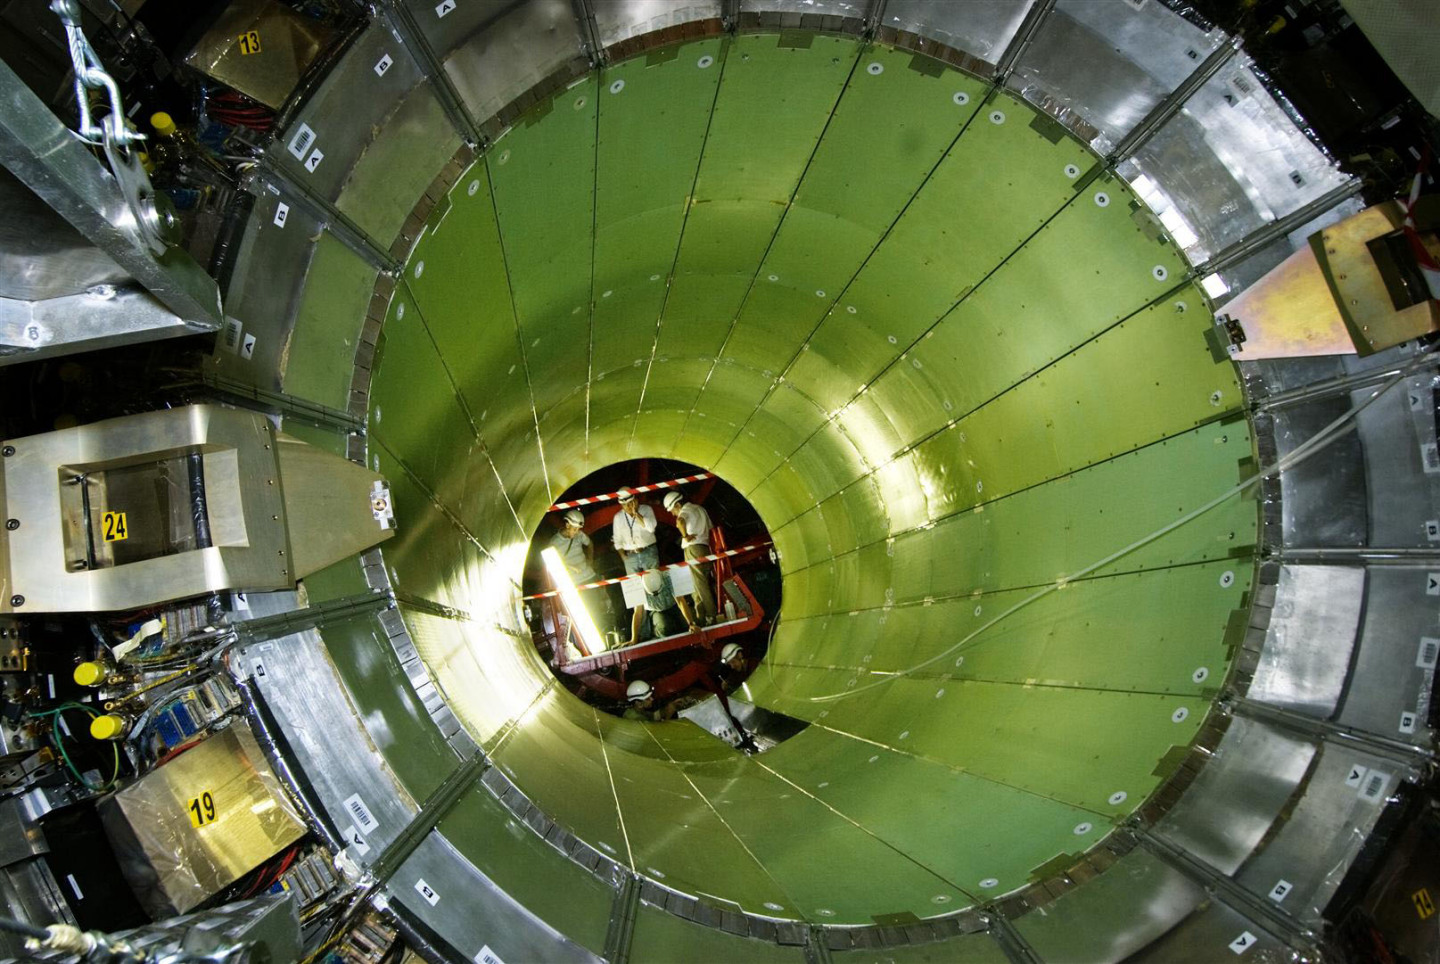
\includegraphics[width=0.8\linewidth]{CMS/EB.jpg}\label{EB}}
	\\
	\subfloat[Un bouchon du ECAL (EE).]{\includegraphics[width=.40\linewidth]{CMS/EE.jpg}\label{EE}}
	\subfloat[Un des preshower du ECAL.]{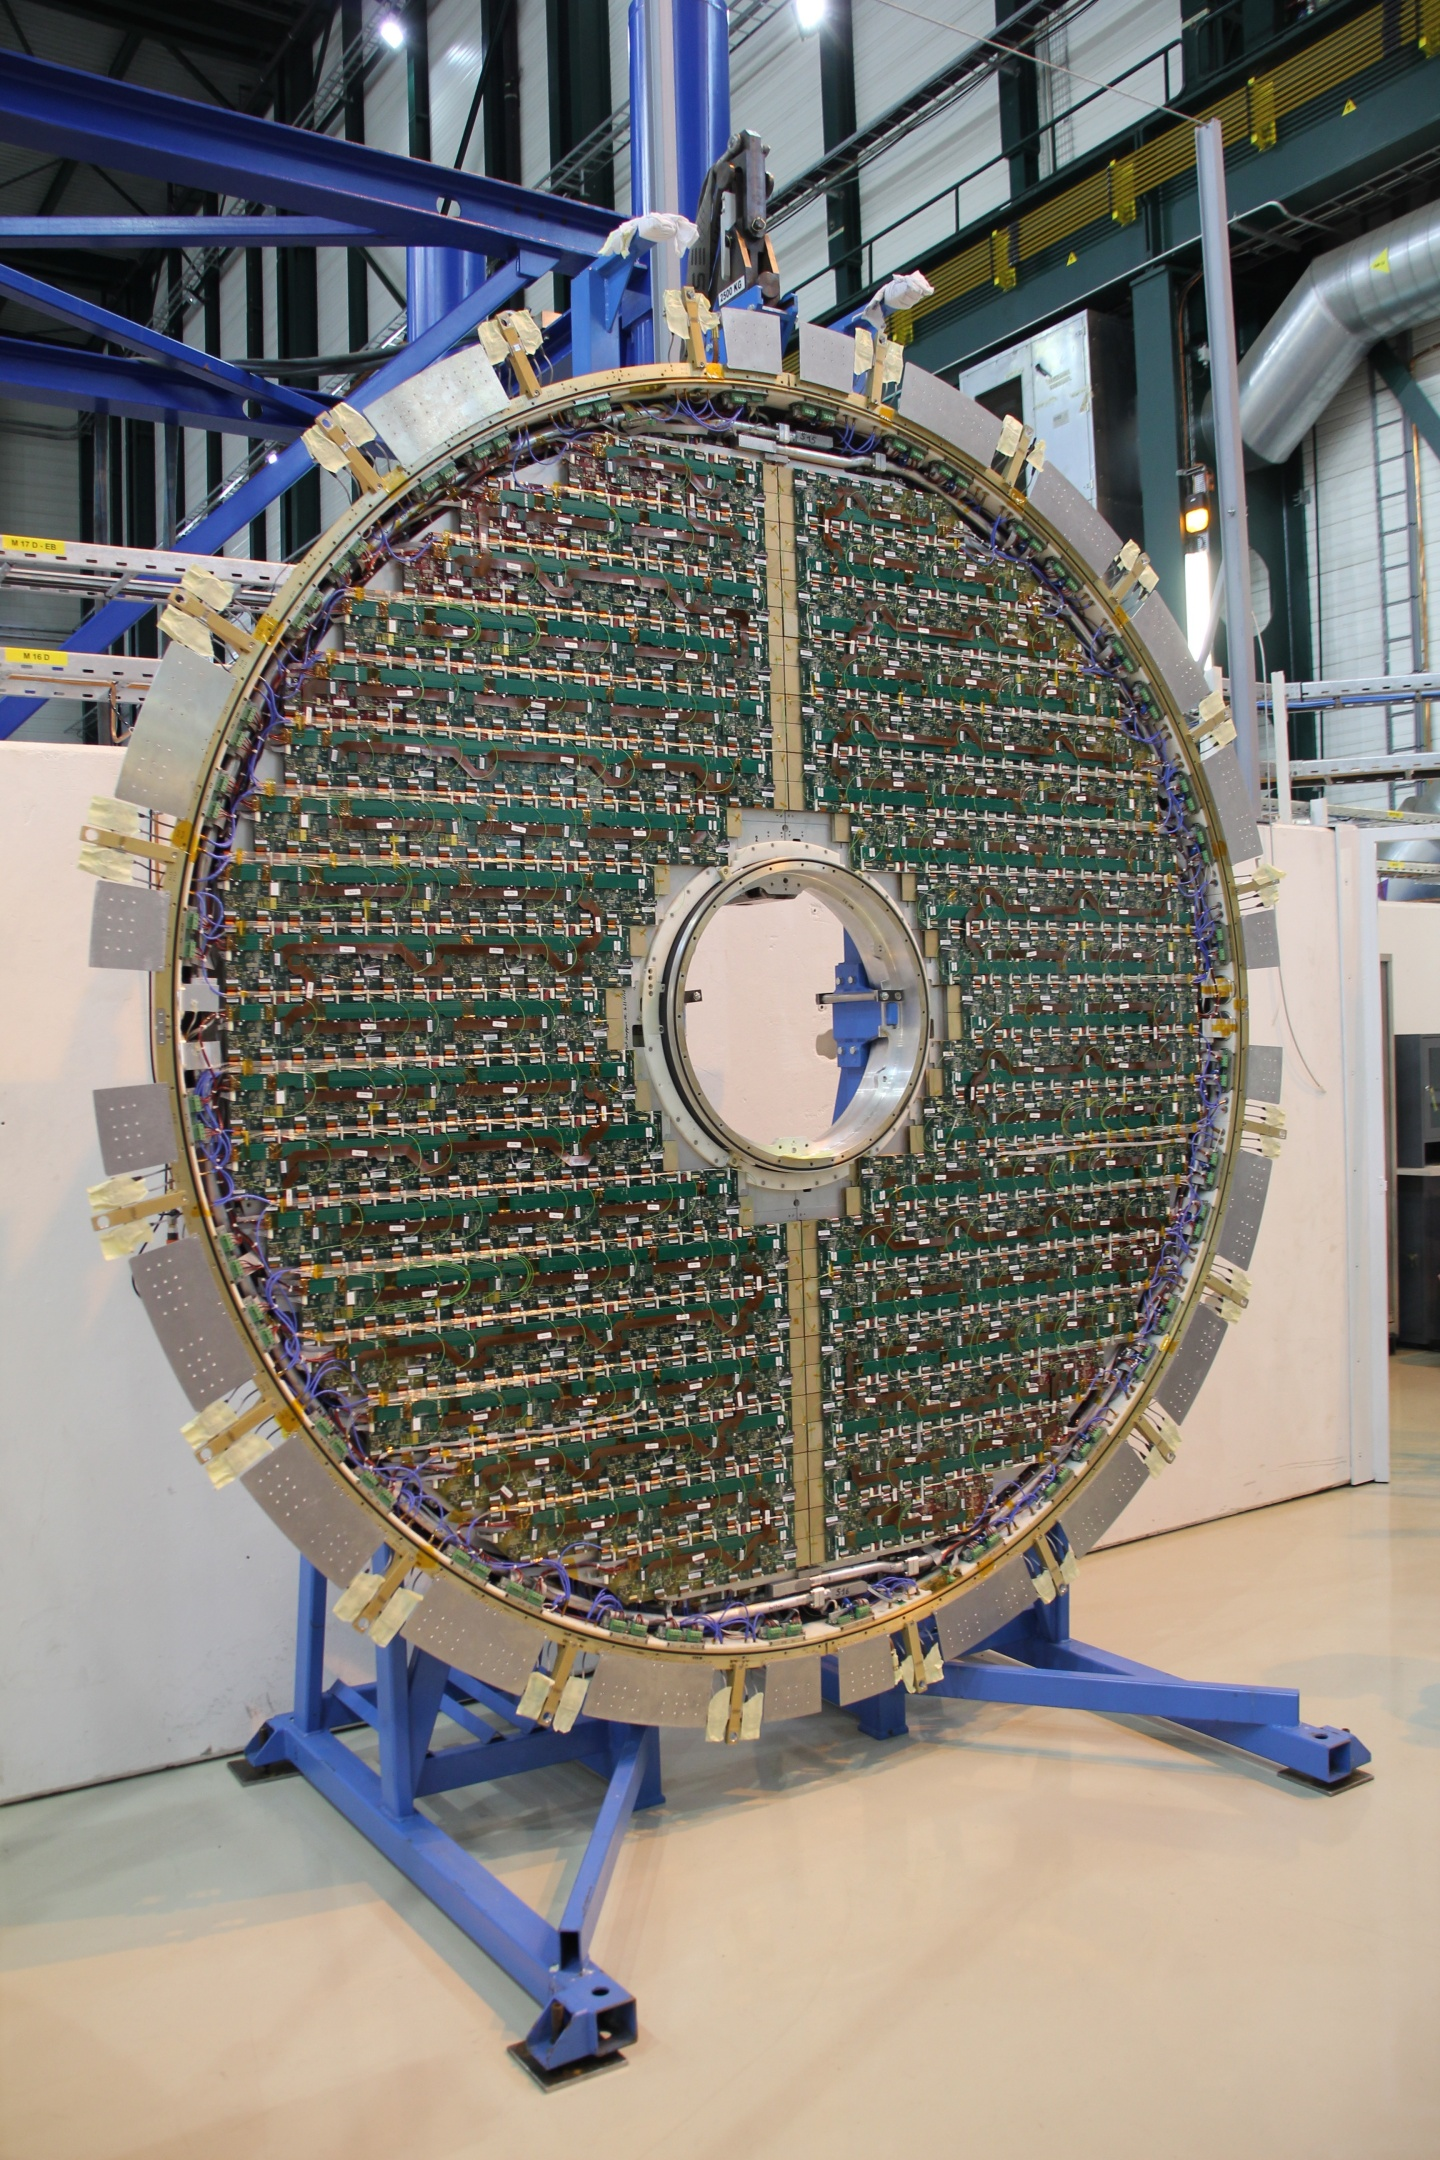
\includegraphics[width=.40\linewidth]{CMS/preshower.jpg}\label{PRESHOWER}}
	\caption{Photos des différents composants du Calorimètre électromagnétique.}
\end{figure}
\subsection{Le calorimètre hadronique}
	\marginpar
{
	\centering
	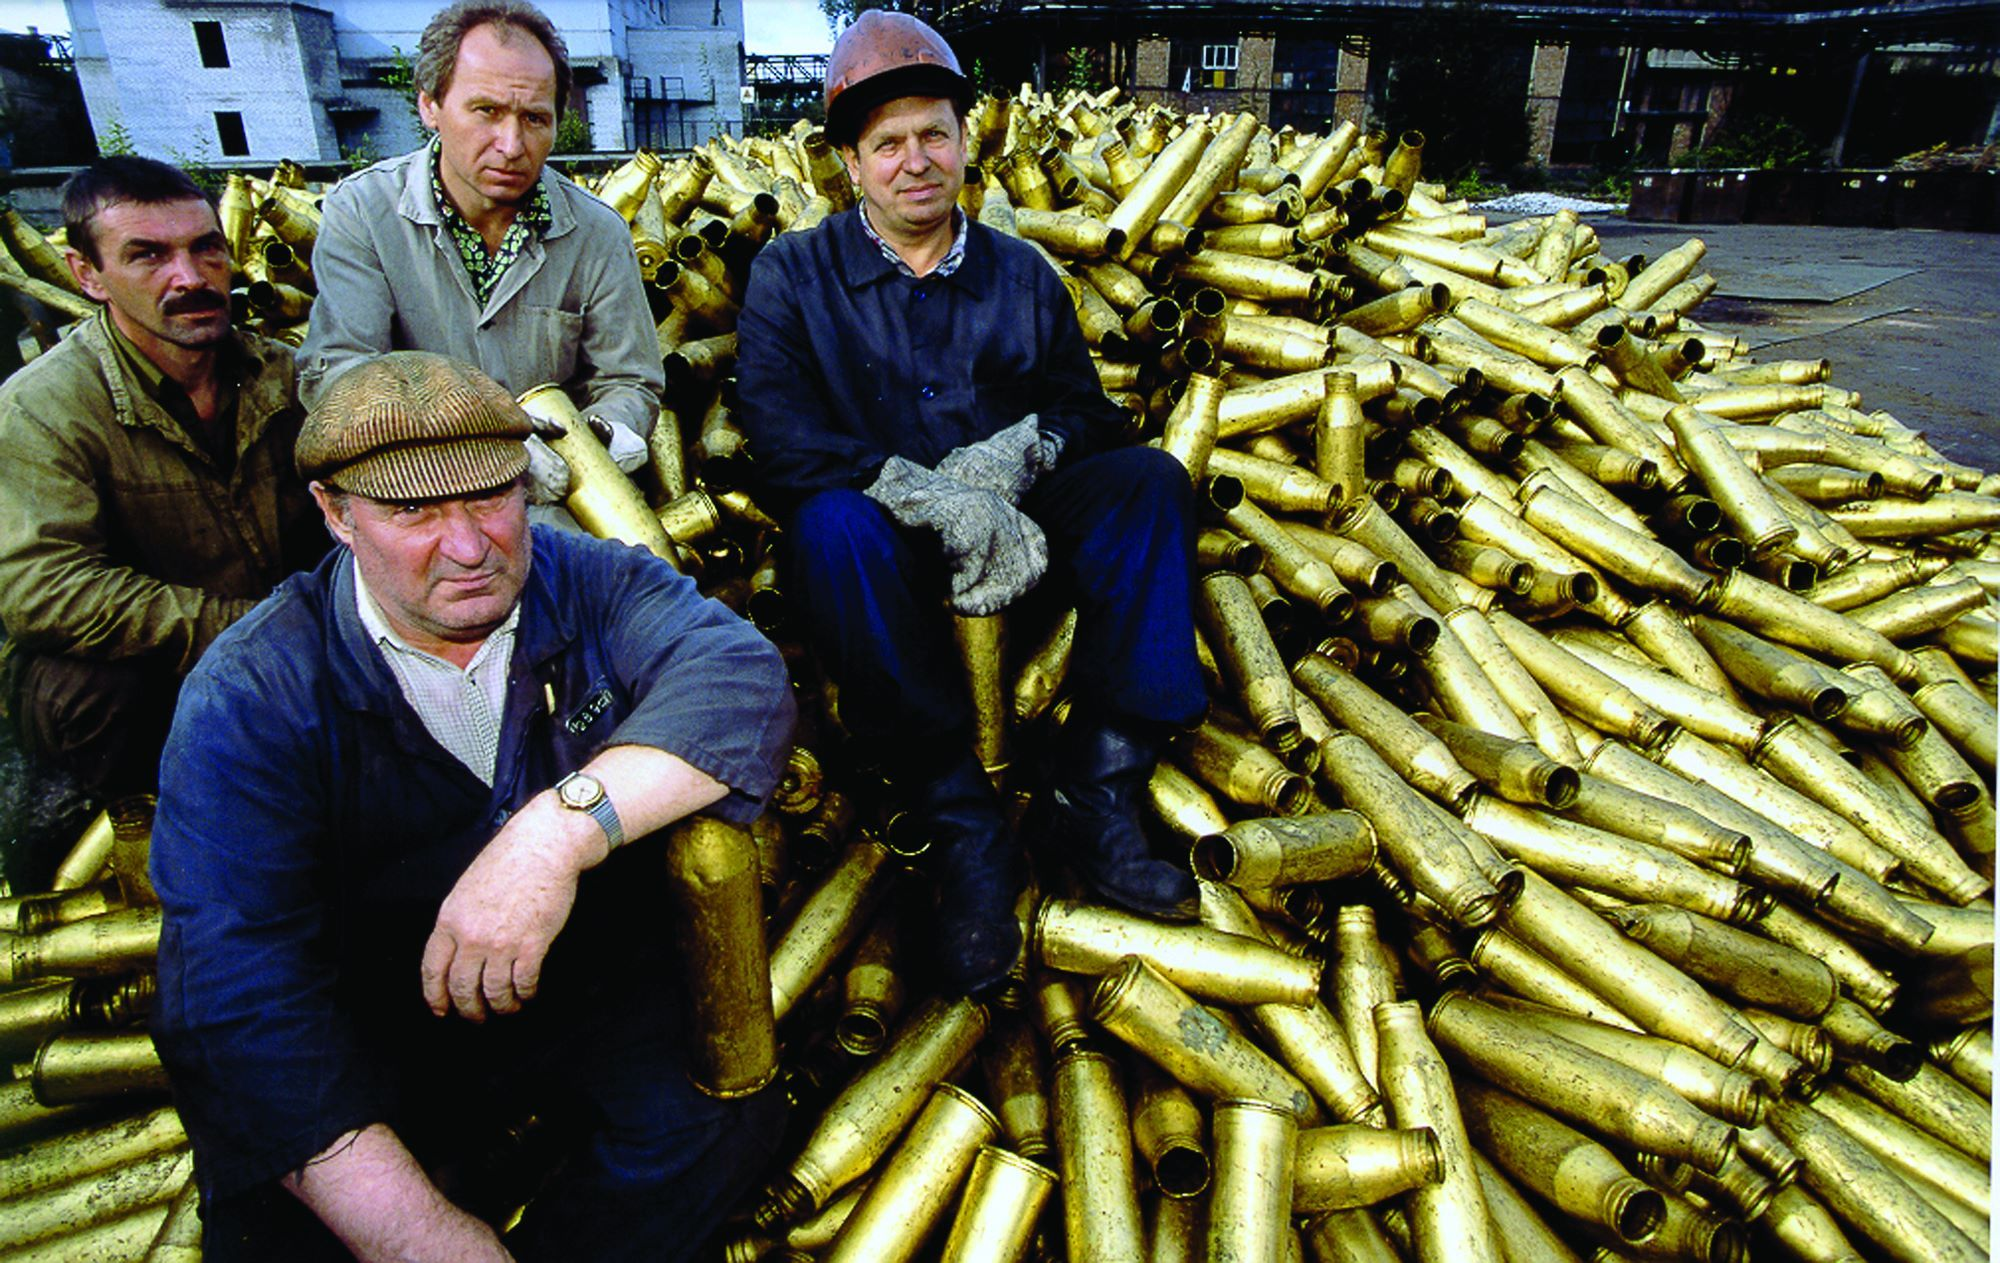
\includegraphics[width=\marginparwidth]{CMS/LAITON.jpg}
	\captionof{figure}{Photo de douilles de la marine russe réutilisées pour la construction du HCAL.}
	\label{LAITON}
}
	\marginpar
{
	\centering
	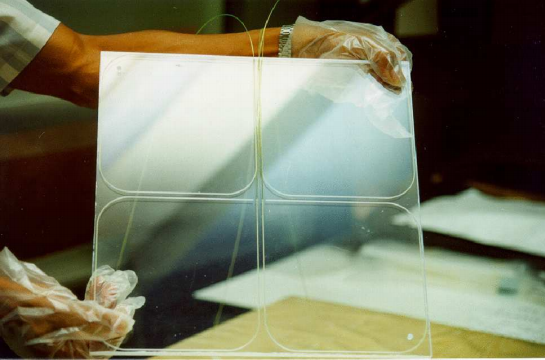
\includegraphics[width=\marginparwidth]{CMS/SCINTI.png}
	\captionof{figure}{Photo d'une tuile du HO avec des fibres WLS insérées dans les 4 $\sigma$-rainures.}
	\label{SCINTI}
}
\marginpar
{
	\centering
	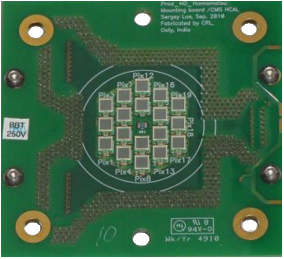
\includegraphics[width=\marginparwidth]{CMS/MPPC.png}
	\captionof{figure}{Photo d'un MPPC.}
	\label{MPPC}
}
\marginpar
{
	\centering
	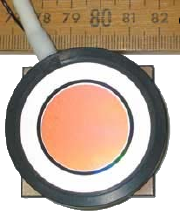
\includegraphics[width=\marginparwidth]{CMS/HPD.png}
	\captionof{figure}{Photo d'une HPD.}
	\label{HPD}
}
Le calorimètre hadronique de CMS ou \textit{Hadronic CALorimeter} (HCAL) (cf.fig\ref{HCAL}) permet de mesurer l'énergie et la direction des hadrons issus de l'hadronisation des quarks et gluons produits lors des collisions. Ce détecteur à une grande compacité spatiale et énergétique et est très compact car il se trouve pour une grande partie entre le ECAL et l'aimant supraconducteur. Cette disposition a nécessité de maximiser la quantité d'absorbeur et de minimiser les parties actives du détecteur. L'absorbeur est constitué de laiton (cf.fig\ref{LAITON}) qui possède une faible longueur d'interaction $\lambda_{l}$ et un faible taux de diffusions multiples. Les hadrons perdent majoritairement leur énergie par interaction nucléaire avec l'absorbeur. La plupart des hadrons sont stoppés avec 9$\lambda_{l}$. Le laiton est également non magnétique ce qui est nécessaire vu l'emplacement du calorimètre. Le matériau actif est composé de feuilles de scintillateurs fluorescents (cf.fig\ref{SCINTI}). La scintillation est ensuite récoltée par des fibre optique qui décale la longueur d'onde de la lumière (WLS). Le signal est ensuite lu par des Multi-Pixel Photon Counter (MPPC) (cf.fig\ref{MPPC}) pour le sous-détecteur Hadronic Outward calorimeter et par des photodiodes hybrides (HPD) (cf.fig\ref{HPD}) pour les autres sous-détecteurs.
\begin{figure}[ht!]
	\centering
	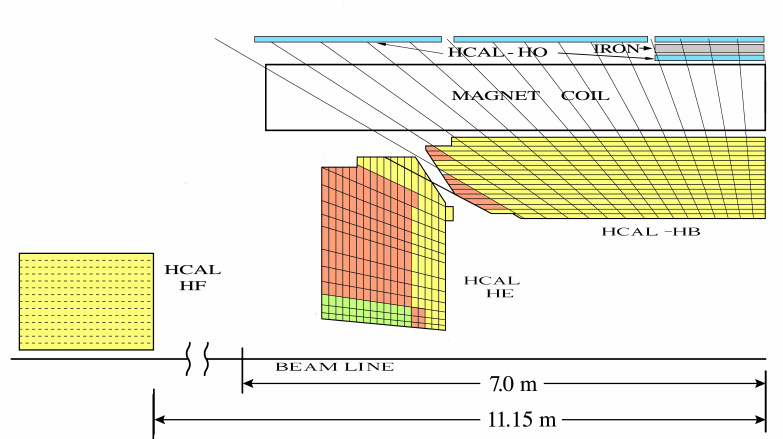
\includegraphics[width=0.95\textwidth]{CMS/HCALSCHEME.png}
	\captionof{figure}{Schéma d'un quart d'une coupe du HCAL de CMS.}
	\label{HCAL}
\end{figure}

Le calorimètre hadronique couvre une zone en pseudo-rapidité jusqu'à $|\eta|<5.0$. Il possède plus de 70000 feuilles de scintillateurs. Il est composé de 4 sous-détecteurs subdividsés en tours : 
\begin{itemize}[label=$\bullet$]
	\item \textbf{Le tonneau} HB pour \textit{Hadronic Barrel calorimeter} (cf.fig\ref{HB}) couvre la région en pseudo rapidité $|\eta|<1.3$. Il est constitué de 36 quartiers couvrant 20 degrés en $\phi$ découpé en quatre sous secteurs de 5 degrés en $\phi$ et 16 sous secteurs en $\eta$. Un quartier possède 16 couches qui sont des empilements de scintillateurs de 9mm d'épaisseur pour les couches les plus externes et 3.7mm pour les autres et d'absorbeur (40 mm de fer pour la première couche, 50.5mm de laiton pour les huit suivantes, 56.5 mm de laiton pour les six suivantes et 75 mm de fer pour la dernière). Les tours ont une segmentation de $\Delta\eta\times\Delta\phi=0.087\times0.087$.
	\item \textbf{Les deux bouchons} HE pour \textit{Hadronic End-cap calorimeter} (cf.fig\ref{HE}) couvrent les régions comprises entre $|\eta|>1.3$ et $|\eta|<3.0$. Une zone inclinée à 53 degrés par rapport à l'axe du faisceau et ne pointant pas vers le point d'interaction est laissée libre afin de permettre le passage des câbles et systèmes nécessaires au trajectographe et au calorimètre électromagnétique. Les bouchons sont segmentés en 18 quartiers de 20 degrés en $\phi$ chacun composé de 14 tours en $\eta$. Les tours sont des empilements de scintillateurs de 3.7 mm d'épaisseur et d'une couche d'absorbeur (9mm pour la premiere couche et 7.5mm pour les suivantes). Une tour possède 19 couches de  scintillateurs en tout; les 5 tours couvrant $|\eta|<1.74$ ont une segmentation de $\Delta\eta\times\Delta\phi=0.087\times0.087$ alors que les 8 couvrant $1.74<|\eta|<3.0$ ont des segmentations allant de $\Delta\eta\times\Delta\phi=0.09\times0.174$ à $\Delta\eta\times\Delta\phi=0.35\times0.174$.
	\item \textbf{Le calorimètre externe} HO pour \textit{Hadronic Outward calorimeter} (cf.fig\ref{HO}) est placé à l'extérieur de l'aimant supraconducteur. Il est constitué de couches de scintillateurs de 10 mm d'épaisseur et couvre la région $|\eta|<1.26$. Ce sous-détecteur permet de récupérer l'énergie sortant du HB et assure une longueur d'interaction de plus de 10$\lambda_{l}$. Le HO est composé de 5 anneaux de 2.536m de long selon $z$ 
	numérotés -2,-1,0,+1,+2 et de centre $z=-5.324, 2.686, 0, 2.686 $et$ 5.324m$ respectivement. Le premier anneau est composé de deux couches de scintillateurs de 10 mm d'épaisseur placées en r=3.82 m et 4.07 m. Les autres anneaux ne possèdent qu'une couche de scintillateur placé à r=4.07 m. Chaque anneau est segmenté en 12 secteurs en $\phi$. Et chaque secteur est segmenté en 8, 6 et 5 tuiles de scintillateurs (cf.fig\ref{SCINTI}) pour les anneaux 0, $\pm1$, $\pm2$ respectivement.
	\item \textbf{Les calorimètres très à l'avant} HF pour \textit{Hadronic Forward calorimeter} couvrent une zone en pseudo-rapidité comprise entre $|\eta|>3.0$ et $|\eta|<5.0$ et $12.5<r<130cm$. Ils sont situés à une distance $|z|=11.2m$ et font 1.65m de long. Ils consistent en un absorbeur de fer qui intègre des fibres de quarks résistantes aux radiations qui assurent la collection rapide de la lumière Cherenkov. La moitié de ces fibres font toute la longueur du détecteur (1.65m) alors que d'autres commencent à 22 cm (soit 143 cm de long) du bord placé vers l'intérieur de CMS. Elles sont placées alternativement à une distance de 5 mm l'une de l'autre en $r$  avec segmentation de $\Delta\eta\times\Delta\phi=0.175\times0.175$. Cette différence de longueur permet de séparer les cascades électromagnétiques des cascades hadroniques. La lumière est ensuite collectée par des tubes photo-multiplicateur (PMT). Le HF est composé de 18 secteur de 20 degrés en $\phi$. Chaque secteur comporte 13 anneaux en $\eta$.
\end{itemize}
\begin{figure}[ht!]
\centering
\subfloat[Le tonneau du HCAL (HB).]{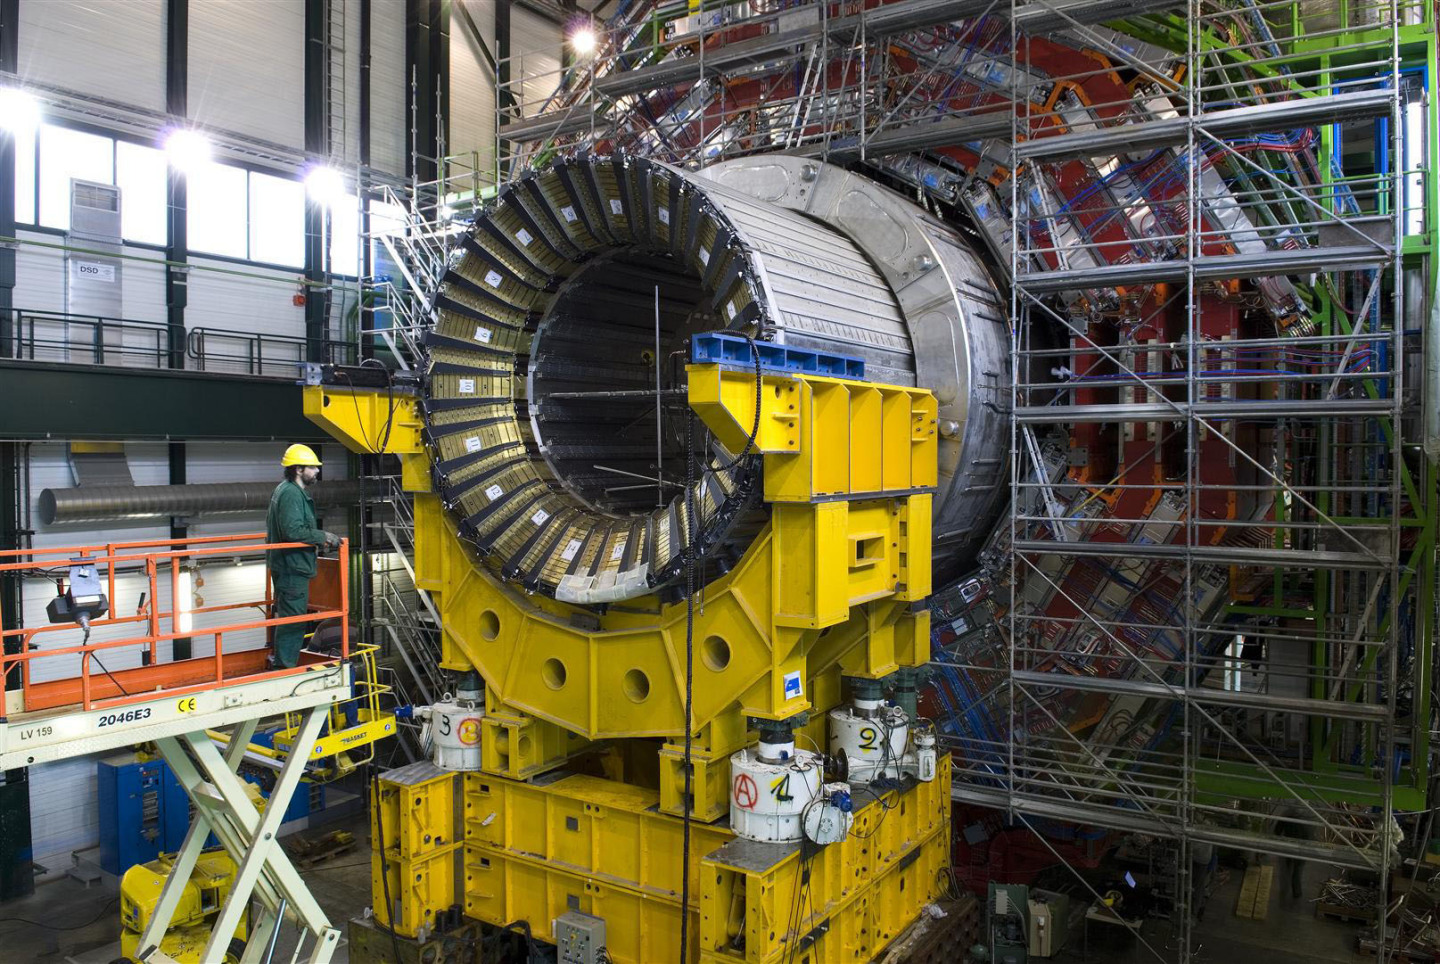
\includegraphics[width=.40\linewidth]{CMS/HB.jpg}\label{HB}}
\subfloat[Un bouchon du HCAL (HE).]{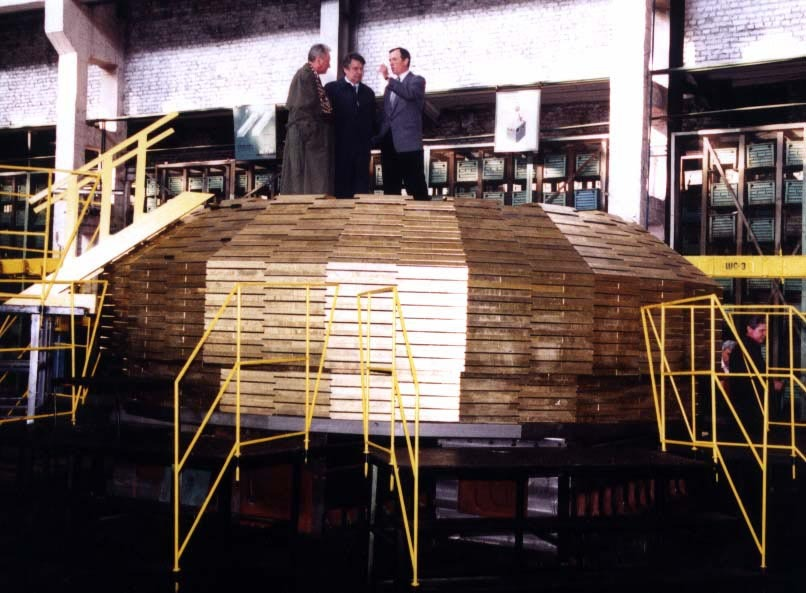
\includegraphics[width=.40\linewidth]{CMS/HE.jpg}\label{HE}}
\\
\subfloat[Installation du HO.]{\includegraphics[width=.40\linewidth]{CMS/HO.jpg}\label{HO}}
%http://cms.desy.de/e53612/e155171/e155181/
\subfloat[Un des HF du HCAL.]{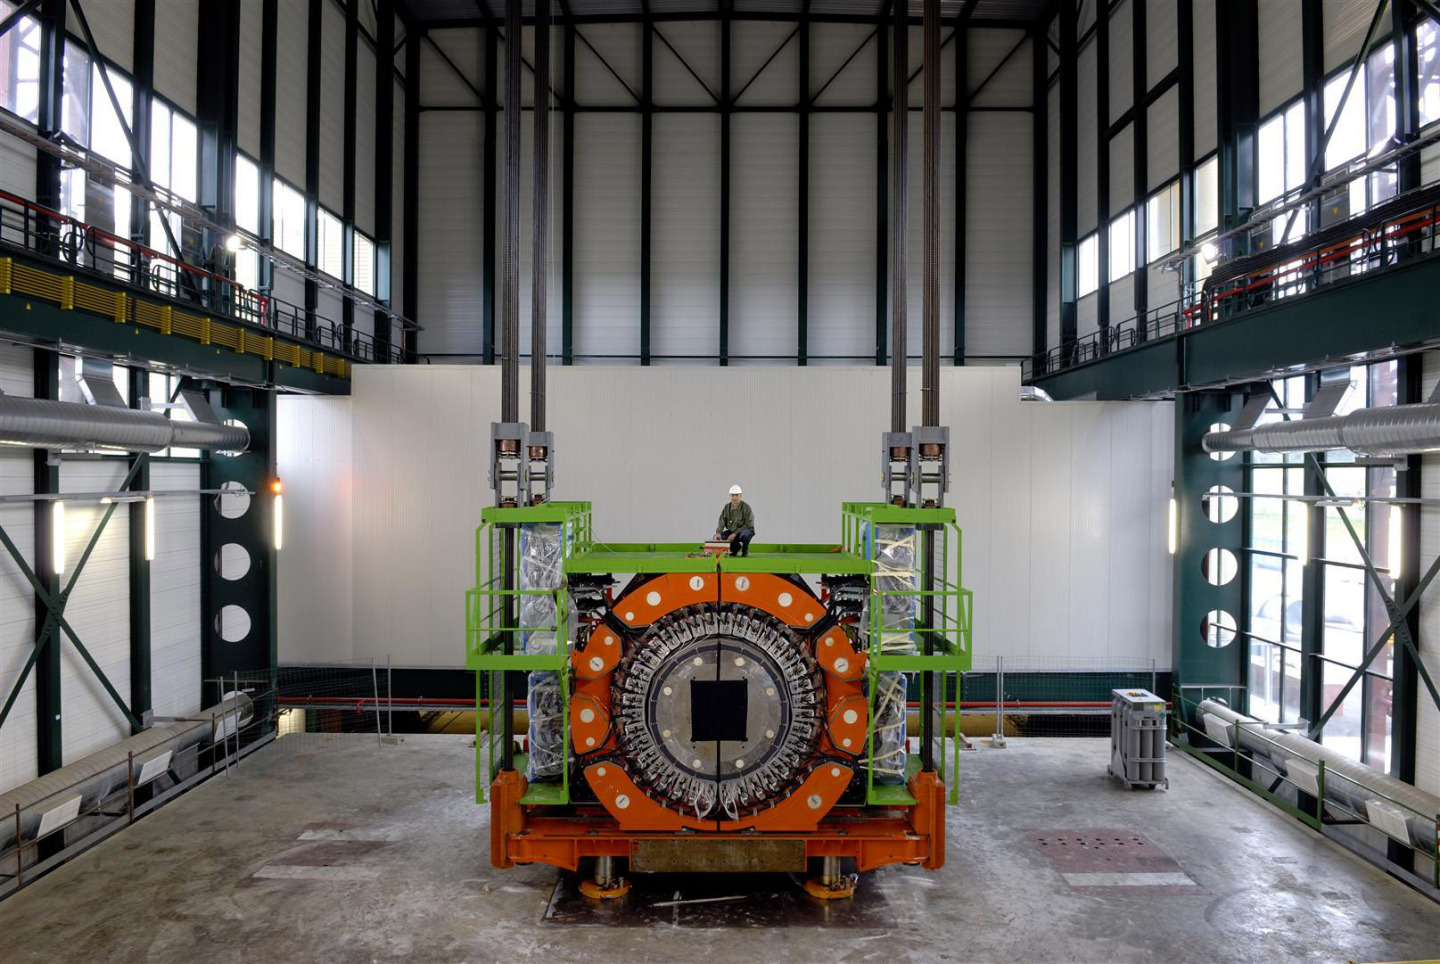
\includegraphics[width=.40\linewidth]{CMS/HF.jpg}\label{HF}}
\caption{Photos des différents composants du calorimètre hadronique.}
\end{figure}	
\subsection{L'aimant supraconducteur}
L'aimant supraconducteur de CMS (cf.fig\ref{MAGNET}) est un solénoïde de 5.9 m de diamètre pour 12.9 m de longueur qui a été prévu pour créer un champ magnétique de 4 T à un courant de 19.14 kA. A pleine puissance, il stocke une énergie de 2.7 GJ. Il est composé de 5 bobines en nobium-titane composées de 2168 spires, refroidies à une température de 4.2 K par de l'hélium liquide. Une structure de retour de champ en fer de 11500 t, composée de 5 culasses (cf.fig\ref{CULASSE}) et 2 bouchons, chacun composé de 3 disques, l'entoure et sert de structure de maintien des chambres à muons. L'épaisseur totale du retour est d'environ 1.5 m (l'épaisseur du troisième disque des bouchons et du premier anneau du tonneau est de 30 cm) et les autres disques des bouchons ainsi que les deuxième et troisième anneaux du tonneau font 60 cm. L'épaisseur à été étudiée afin d'être suffisante pour absorber les hadrons qui traverseraient les calorimètres et l'aimant tout en restant assez fin pour éviter les pertes radiatives pour les muons.
\marginpar
{
	\centering
	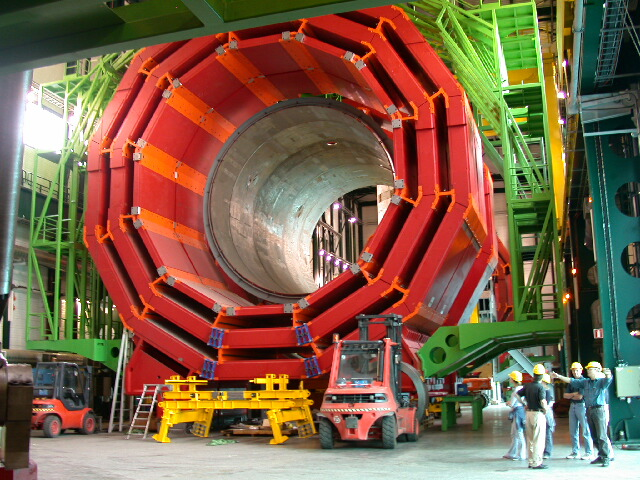
\includegraphics[width=\marginparwidth]{CMS/CULASSE.jpg}
	\captionof{figure}{Photo d'une Cullasse.}
	\label{CULASSE}
}
\begin{figure}[ht!]
	\centering
	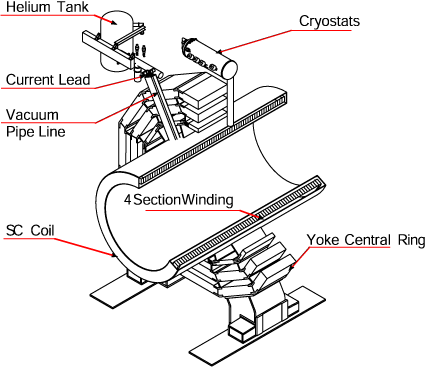
\includegraphics[width=0.50\textwidth]{CMS/MAGNET.png}
	\captionof{figure}{Schéma de l'aimant supra-conducteur de CMS.}
	\label{MAGNET}
\end{figure}
\newpage
La figure \ref{CHAMP} montre une simulation par éléments-finis de la valeur du champ magnétique en fonction de la position.
\begin{figure}[ht!]
	\centering
	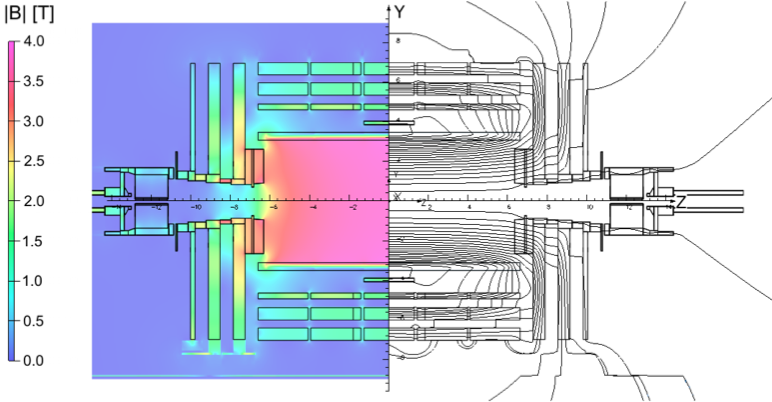
\includegraphics[width=0.90\textwidth]{CMS/CHAMP.png}
	\captionof{figure}{Valeur du champ magnétique (gauche) et lignes de champ (droite) selon une coupe longitudinale du détecteur CMS, prédits par la simulation. Pour une valeur du champ central de 3.8 T.}
	\label{CHAMP}
\end{figure}
\subsection{Le spectrographe à muons}

Le spectographe à muons (cf.fig\ref{CMS1},fig\ref{CMS2}) a pour but d'identifier les muons, de mesurer avec précision leur quantité de mouvement et de déclencher sur les événements contenant des muons.
\marginpar
{
	\centering
	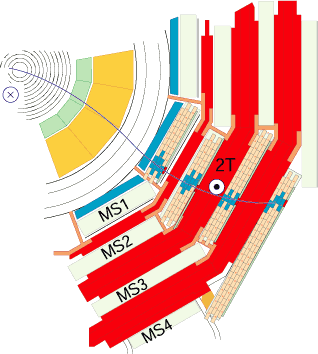
\includegraphics[width=\marginparwidth]{CMS/MUON.png}
	\captionof{figure}{Quart d'une coupe dans le plan transverse du détecteur CMS montrant la trajectoire d'un muon (courbe bleue).}
	\label{MUON}
} Les muons ont un très grand pouvoir de pénétration. Il est donc possible d'utiliser à la fois les traces chargées laissées dans le trajectographe et dans des détecteurs placés après l'aimant pour les identifier et les reconstruire de manière précise. Une bonne résolution de la quantité de mouvement des muons et leur bonne identification est obtenue grâce au champ magnétique intense de l'aimant et du retour de champ dans la culasse qui assure une trajectoire avec une double courbure. Cette culasse doit contenir des détecteurs de grande taille afin d'augmenter la probabilité de détection; ils faut donc qu'ils soient peu onéreux et fiables. Il faut également que ces détecteurs ne soient pas atteints par d'autres particules afin d'assurer un signal propre, pour ce faire la distance depuis l'aimant jusqu'à la dernière station du spectrographe et de l'ordre de 16 longueurs de radiation, ce qui évite le bruit de fond hadronique résiduel venant du faisceau.

\begin{sidewaysfigure}
\centering
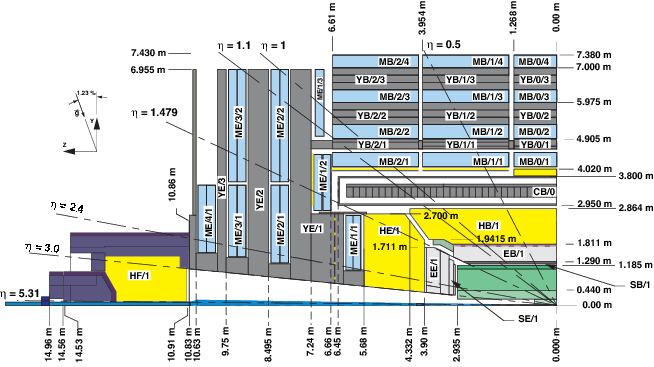
\includegraphics[width=0.80\textwidth]{CMS/CMSLONG.png}
\captionof{figure}{Coupe longitudinale d'un quart de CMS.}
\label{CMS1}
\end{sidewaysfigure}


\begin{figure}[p]
\centering
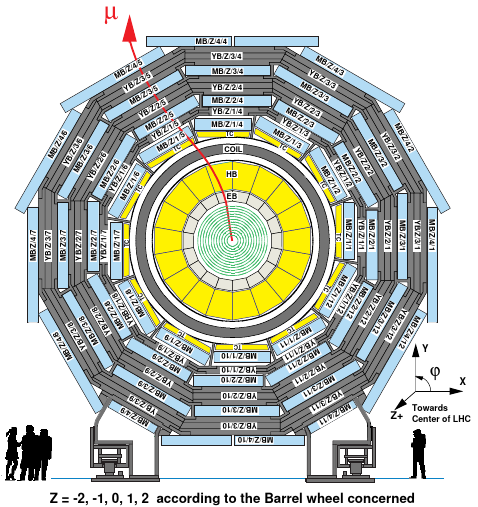
\includegraphics[width=0.98\textwidth]{CMS/CMSTRANS.png}
\captionof{figure}{Coupe transversale de la partie centrale CMS.}
\label{CMS2}
\end{figure}

Le spectographe à muons, est composé de 3 sous-détecteurs :
\begin{itemize}[label=$\bullet$]
	\item \textbf{Les chambres à dérive} DT pour \textit{Drift Tube} (cf.fig\ref{DT}) sont présents seulement dans le tonneau ou le flux de muon est faible tout comme le bruit de font des neutrons; Le champ magnétique est également assez faible (~0.4T) et uniforme. Ce détecteur est constitué de 250 chambres inséré dans la culasse de CMS.Il sont disposés en 4 couches selon r à des distances r=4.0,4.9,5.9 et 7.0m. La culasse est composé selon l'axe $z$ de 5 roues numéroté de -2 à 2, chacune comportant 12 (sauf pour MB4 qui en posséde 14) secteurs dans le plan transverse numéroté à partir de $\phi=0$ couvrant 30 degrees. Ce détecteur couvre une zone en pseudo rapidité $\eta<1.2$. Chaque chambre est constituée de 8 couches de tubes (cf.fig\ref{DT1}) mesurant la courbure de la trajectoire des muons selon $\phi$ est 4 couches pour la courbure selon $\eta$. Chaque ensemble de 4couches est appellé super-couche \textit{superlayer}. Les deux super-couche mesurant $\psi$ sont séparé par 20cm d'aluminium en nid d'abeille. Seul les chambre de MB4 ne possede pas de superlayer mesurant $\eta$ bien que la distance entre les deux superlayer restant reste la même.
	\begin{figure}[ht!]
		\centering
		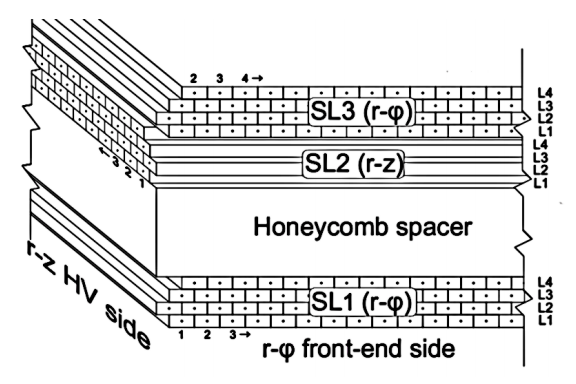
\includegraphics[width=0.50\textwidth]{CMS/DTchamber.png}
		\captionof{figure}{Schéma d'une chambre à dérive.}
		\label{DT1}
	\end{figure}

    Les tubes d'une couche de la chambre sont constitué de 5 électrodes : un fil d'acier inoxydable au centre du tube composant l'anode, 2 pistes servant de cathodes et 2 pistes servant d'électrode et à mettre en forme le champ électrique. Ces deux électrodes améliore l'uniformité du champ à l'intérieur du tube loin du fil et améliore ainsi la résolution spatiale. Le tube est rempli d'un gaz de ArCO2 85/15. Lorsqu'une particule traverse le tube, elle ionise le gaz qui libère des électrons qui sont ensuite accélérer vers l'anode. Une avalanche se crée prêt du fil, ou le champ électrique est intense, ce qui induit un signal sur le fil. Le temps maximal nécessaire à la propagation du signal est de 380ns. 
    
    	\begin{figure}[ht!]
    	\centering
    	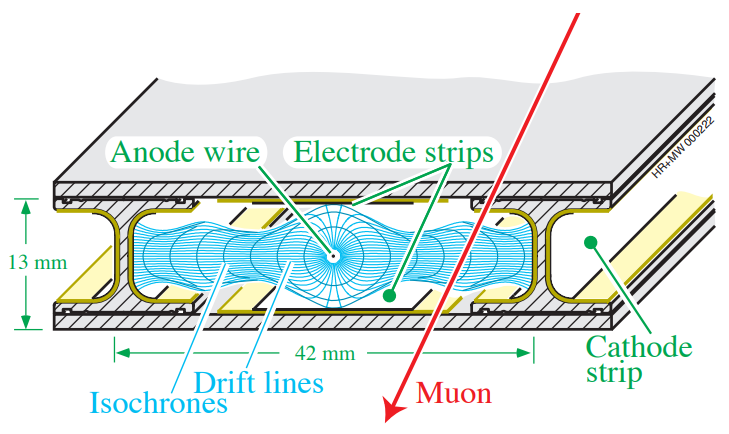
\includegraphics[width=0.50\textwidth]{CMS/DTTUBE.png}
    	\captionof{figure}{Schéma d'un tube d'une chambre à dérive.}
    	\label{DT2}
    	\end{figure}
    En estimant le temps d'arrivée des électrons sur l'anode, en supposant le temps d'interaction connu et en ayant trois couche d'un superlayer touché, il est possible d'estimer la position et le temps de la trace. dans un superlayer une resolution de 20mrad en angle 1.5mm en résolution spatial et quelques ns de résolution temporelle sont atteints.
    
    \item \textbf{Les chambres à pistes cathodiques }CSC pour \textit{Cathode Strip Chambers} (cf.fig\ref{CSC}) sont présent dans les bouchons où le flux de muons ainsi que le bruit de fond sont imoportant, le champ magnétique est également non-uniforme. Ces chambre on un temps de réponse très court, une granularité fine et sont presque insensible à la non-uniformité du champ magnétique. Ce détecteur couvre les zones de pseudo-rapidité $0.9<=|\eta|<=2.4$ et consiste en 468 chambres installé dans les bouchons. Chaque bouchons comprends 4 stations nommé ME1 ME2 ME3 et ME4. chaque stations comprends 2 anneaux (sauf ME1 qui en comprends 3) segmenter en 36 chambres couvrant chacunes un angle de 20degree en $\phi$.
    
    Les chambres (cf.fig\ref{CSC2}) sont cosntitués de 6 couches contenant un mélange de gaz (40\% Ar 50\%CO2 qui assure un bon gain et 10\%CF4 afin d'empecher la polymerisation pret des fils.) ainsi q'un plan de pistes de cathode radiale et de fils séparés de 3mm constituant les anodes placés orthogonalement aux pistes (sauf pour les premier anneaux de ME1 ou les fils sont orienté à 26degree afin de compenser la force de Lorentz du au champ magnétique de 4T dans cette zone). Les nombres total de pistes est de 220 000 et plus de 2 millions de fils.
    
    Lorqu'une particule chargée traverse une CSC, elle ionise le gaz. Les electrons sont accéléré vers le fils à anode. Le mouvement de ces charges induit un signal sur les pistes cathode et les fils anode de la chambre. Le temps dérive est beaucoup plus rapide que pous les DT mais la résolution spatiale est faible : 200um dans le plan tansverse et 10mrad dans le plan longitudinal.
    \begin{figure}[ht!]
    	\centering
    	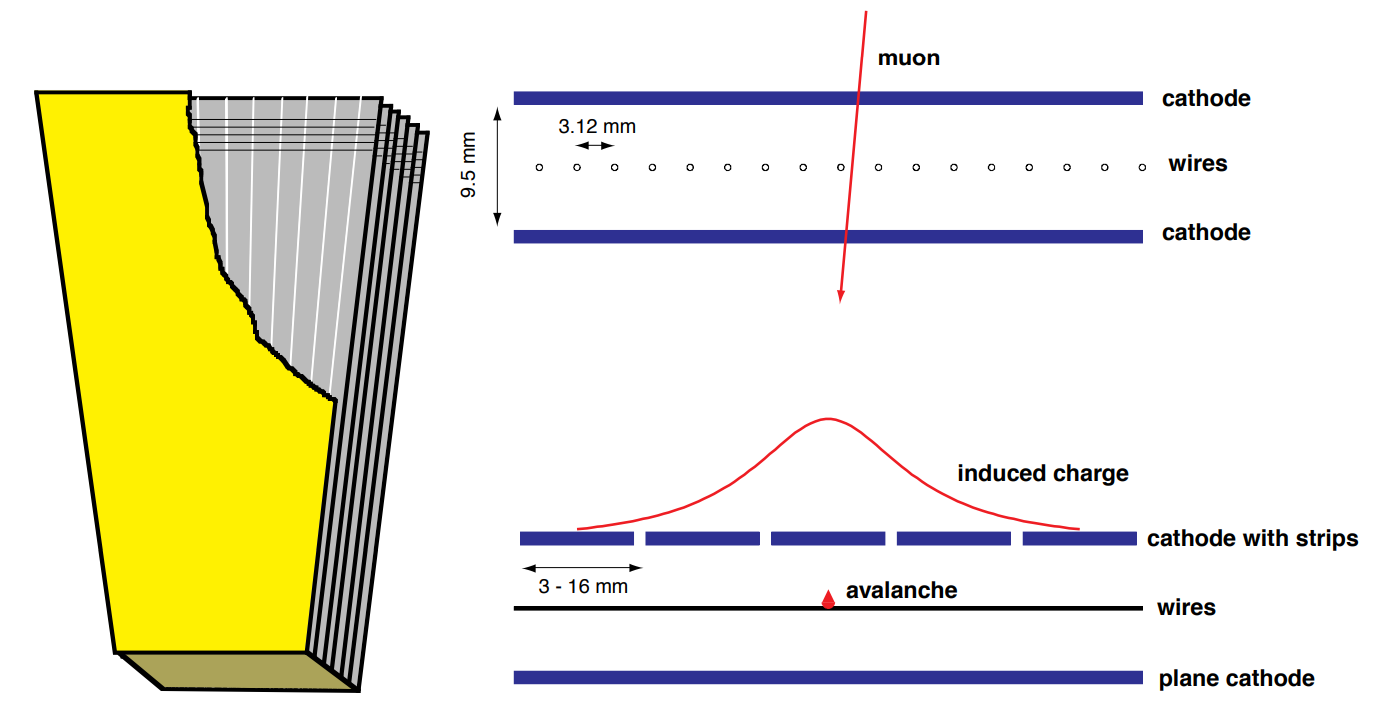
\includegraphics[width=0.50\textwidth]{CMS/CSC2.png}
    	\captionof{figure}{Schéma d'une chambre CSC.}
    	\label{CSC2}
    \end{figure}
    
    
    
	\item \textbf{Les chambres à plaques résistives} RPC pour \textit{Resistive plate Chambers} (cf.fig\ref{RPC}) forment un système très efficace pour trigger sur les muons même à bas $p_{T}$ et sur une zone en pseudo rapidité très large ($|\eta<1.6|$). grâce à sont excellente résolution temporelle (~ns) et compléte les détecteurs CSC et DT dont les résolutions spatiales sont beaucoup plus éleve. Les RPC permettent d'assigner avec une plus grande précision le bon temps de croisement de faisceau pour les muons. Elles sont présentes à la fois dans le tonneaux et les bouchons. Dans le tonneau 480 sont réparti en 6 couches, 2 pour MB1 et MB2 et 1 pour MB3 et MB4. La redondance en MB1 et MB2 permet  de trigger sur les muons de bas $p_{T}$ qui pourrait êttre arrêtés avant d'atteindre MB3. Pour les bouchons, les 432 chambres sont répartis en trois disque noté RE1 RE2 RE3 pour chaque bouchon. Chaque disque est composés de 3 anneaux RE*/1 RE*/2 RE*/3 avec * représentant le numéro du disque. Seul les anneaux 2 et 3 sont instrumentés. Chaque anneaux est ségmenté en 18 chambres couvrant $\phi=20$.
	
	Les RPC sont des chambres à double gap (cf.fig\ref{RPC2}) qui opèrent en mode avalanche afin de fonctionner même à haut rate de particules $~qq centaine de Hz/cm2$. Un gap est constitué de deux plates de bakélite qui servent  dans lequel circule un gaz. Des pistes de lectures sont inséré entre les deux gaps. Le système des RPC dans CMS ainsi que le fonctionnement d'unr RPC est expliqué dans le prochain chapitre.
	  \begin{figure}[ht!]
		\centering
		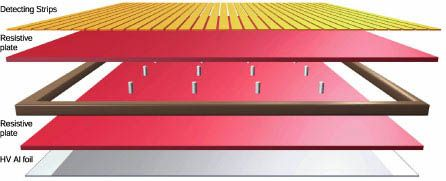
\includegraphics[width=0.60\textwidth]{CMS/RPC2.jpg}
		\captionof{figure}{Schéma en vue éclaté d'un gap d'une RPC et des pistes de lecture.}
		\label{RPC2}
	\end{figure}
	
	
\end{itemize}
    \begin{figure}[ht!]
	\centering
	\subfloat[Photo d'une cassette contenant une chambre DT et RPC.]{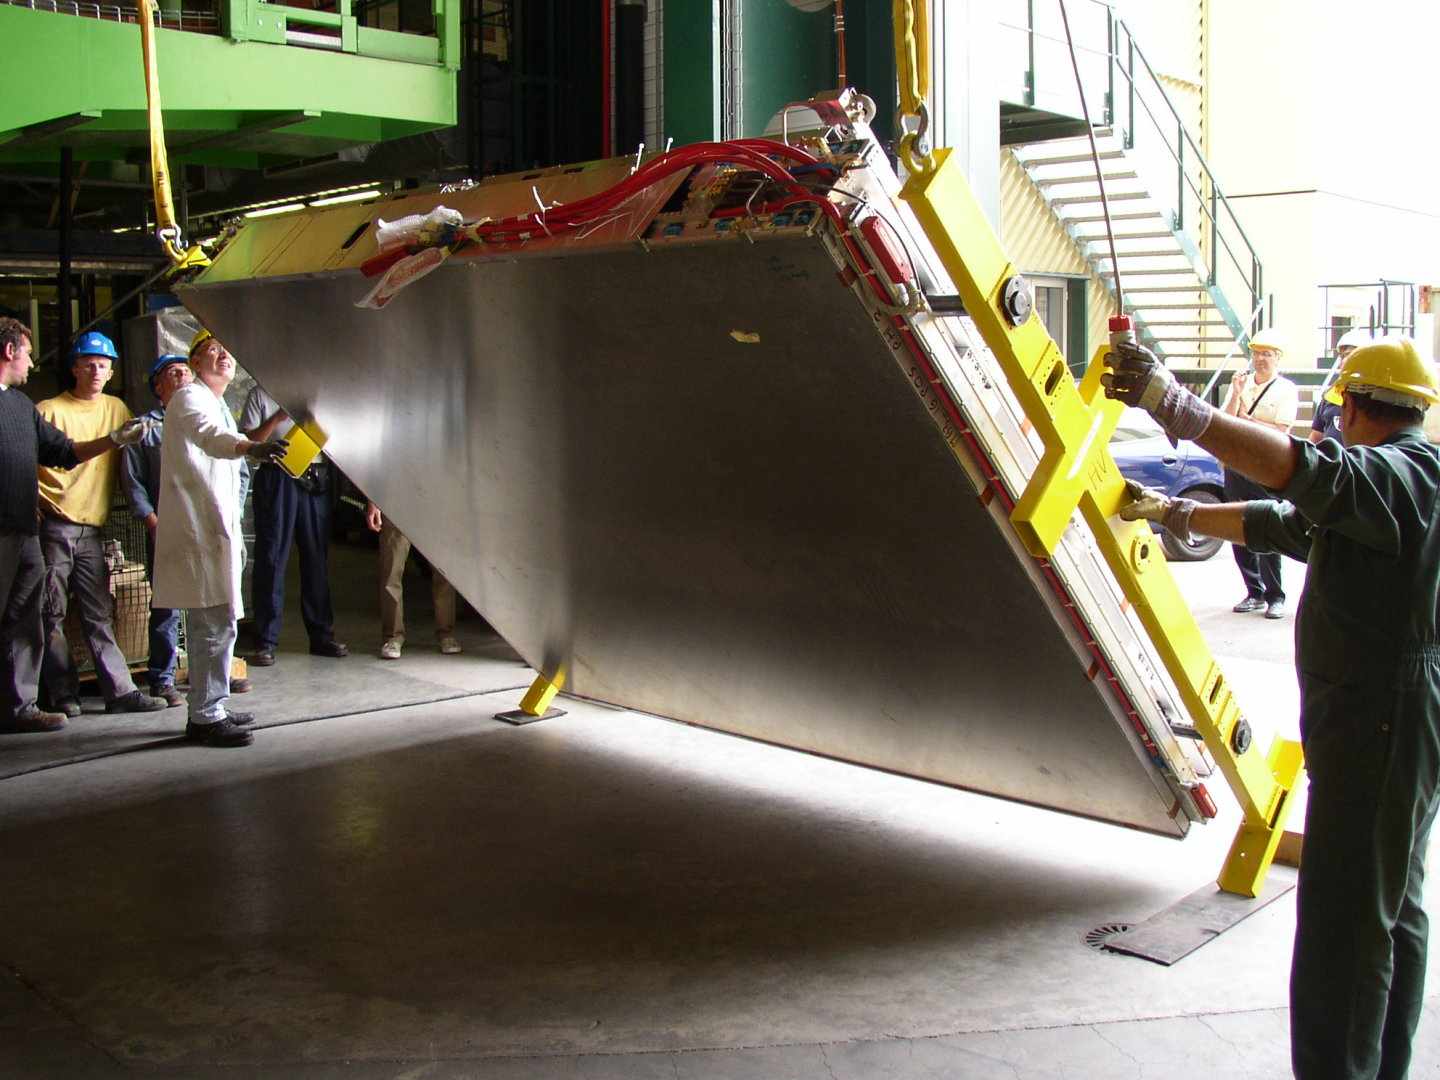
\includegraphics[width=0.40\linewidth]{CMS/DT.jpg}\label{DT}}
	\subfloat[Photo d'une chambre CSC.]{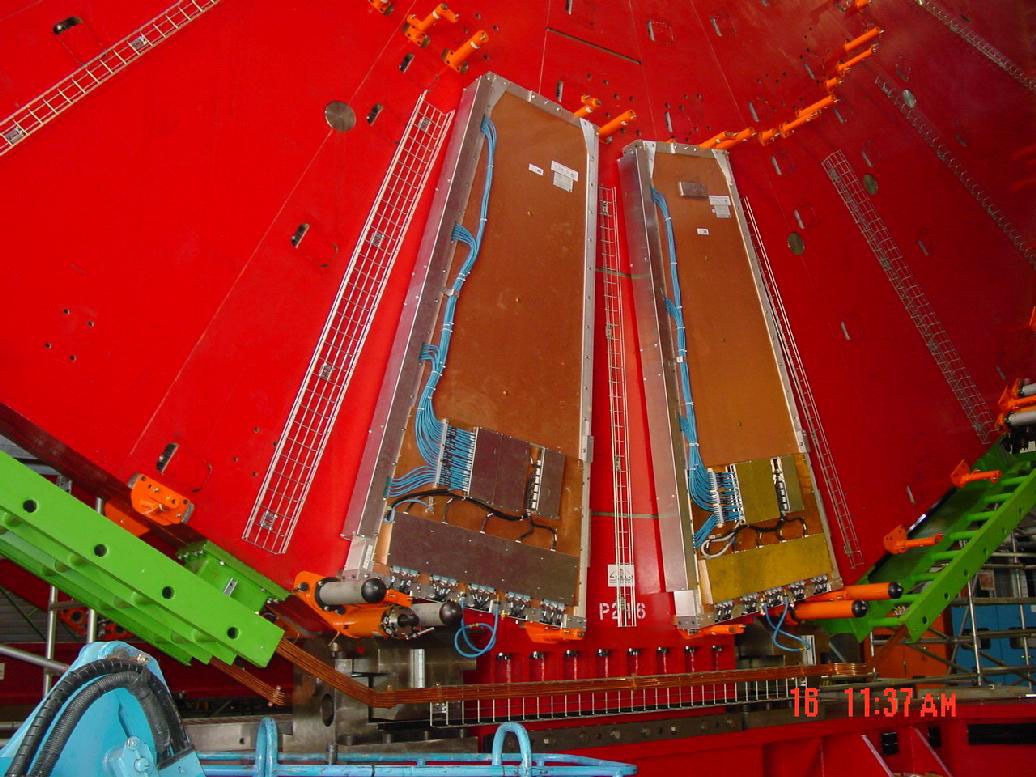
\includegraphics[width=.40\linewidth]{CMS/CSC.jpg}\label{CSC}}
	\\
	\subfloat[Photo d'une chambre RPC.]{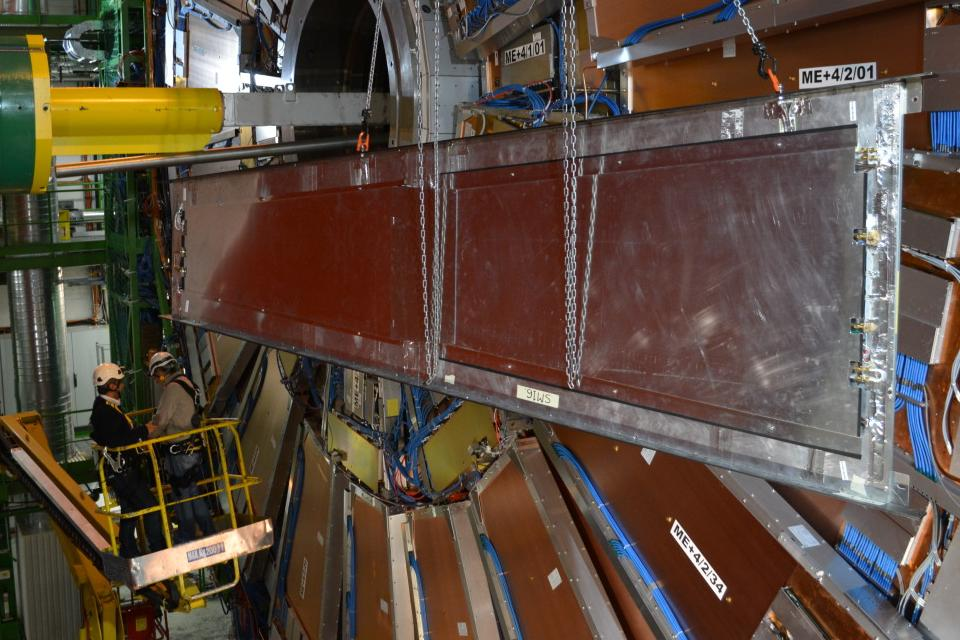
\includegraphics[width=.40\linewidth]{CMS/RPC.jpg}\label{RPC}}
	\caption{Photos des différents composants du spectrographe à muons.}
\end{figure}

\section{Le système de déclenchement et d'acquisition de données}
Chaque types de particules lors de sont passage dans CMS va créer des types de traces particulières qui vont être enregistrer sous forme électronique par les sous-détecteur le composant.La figure \ref{particules} montre une vue schématique des traces laissé par différents types de particules dans les sous-détecteurs de CMS.

	  \begin{figure}[ht!]
	\centering
	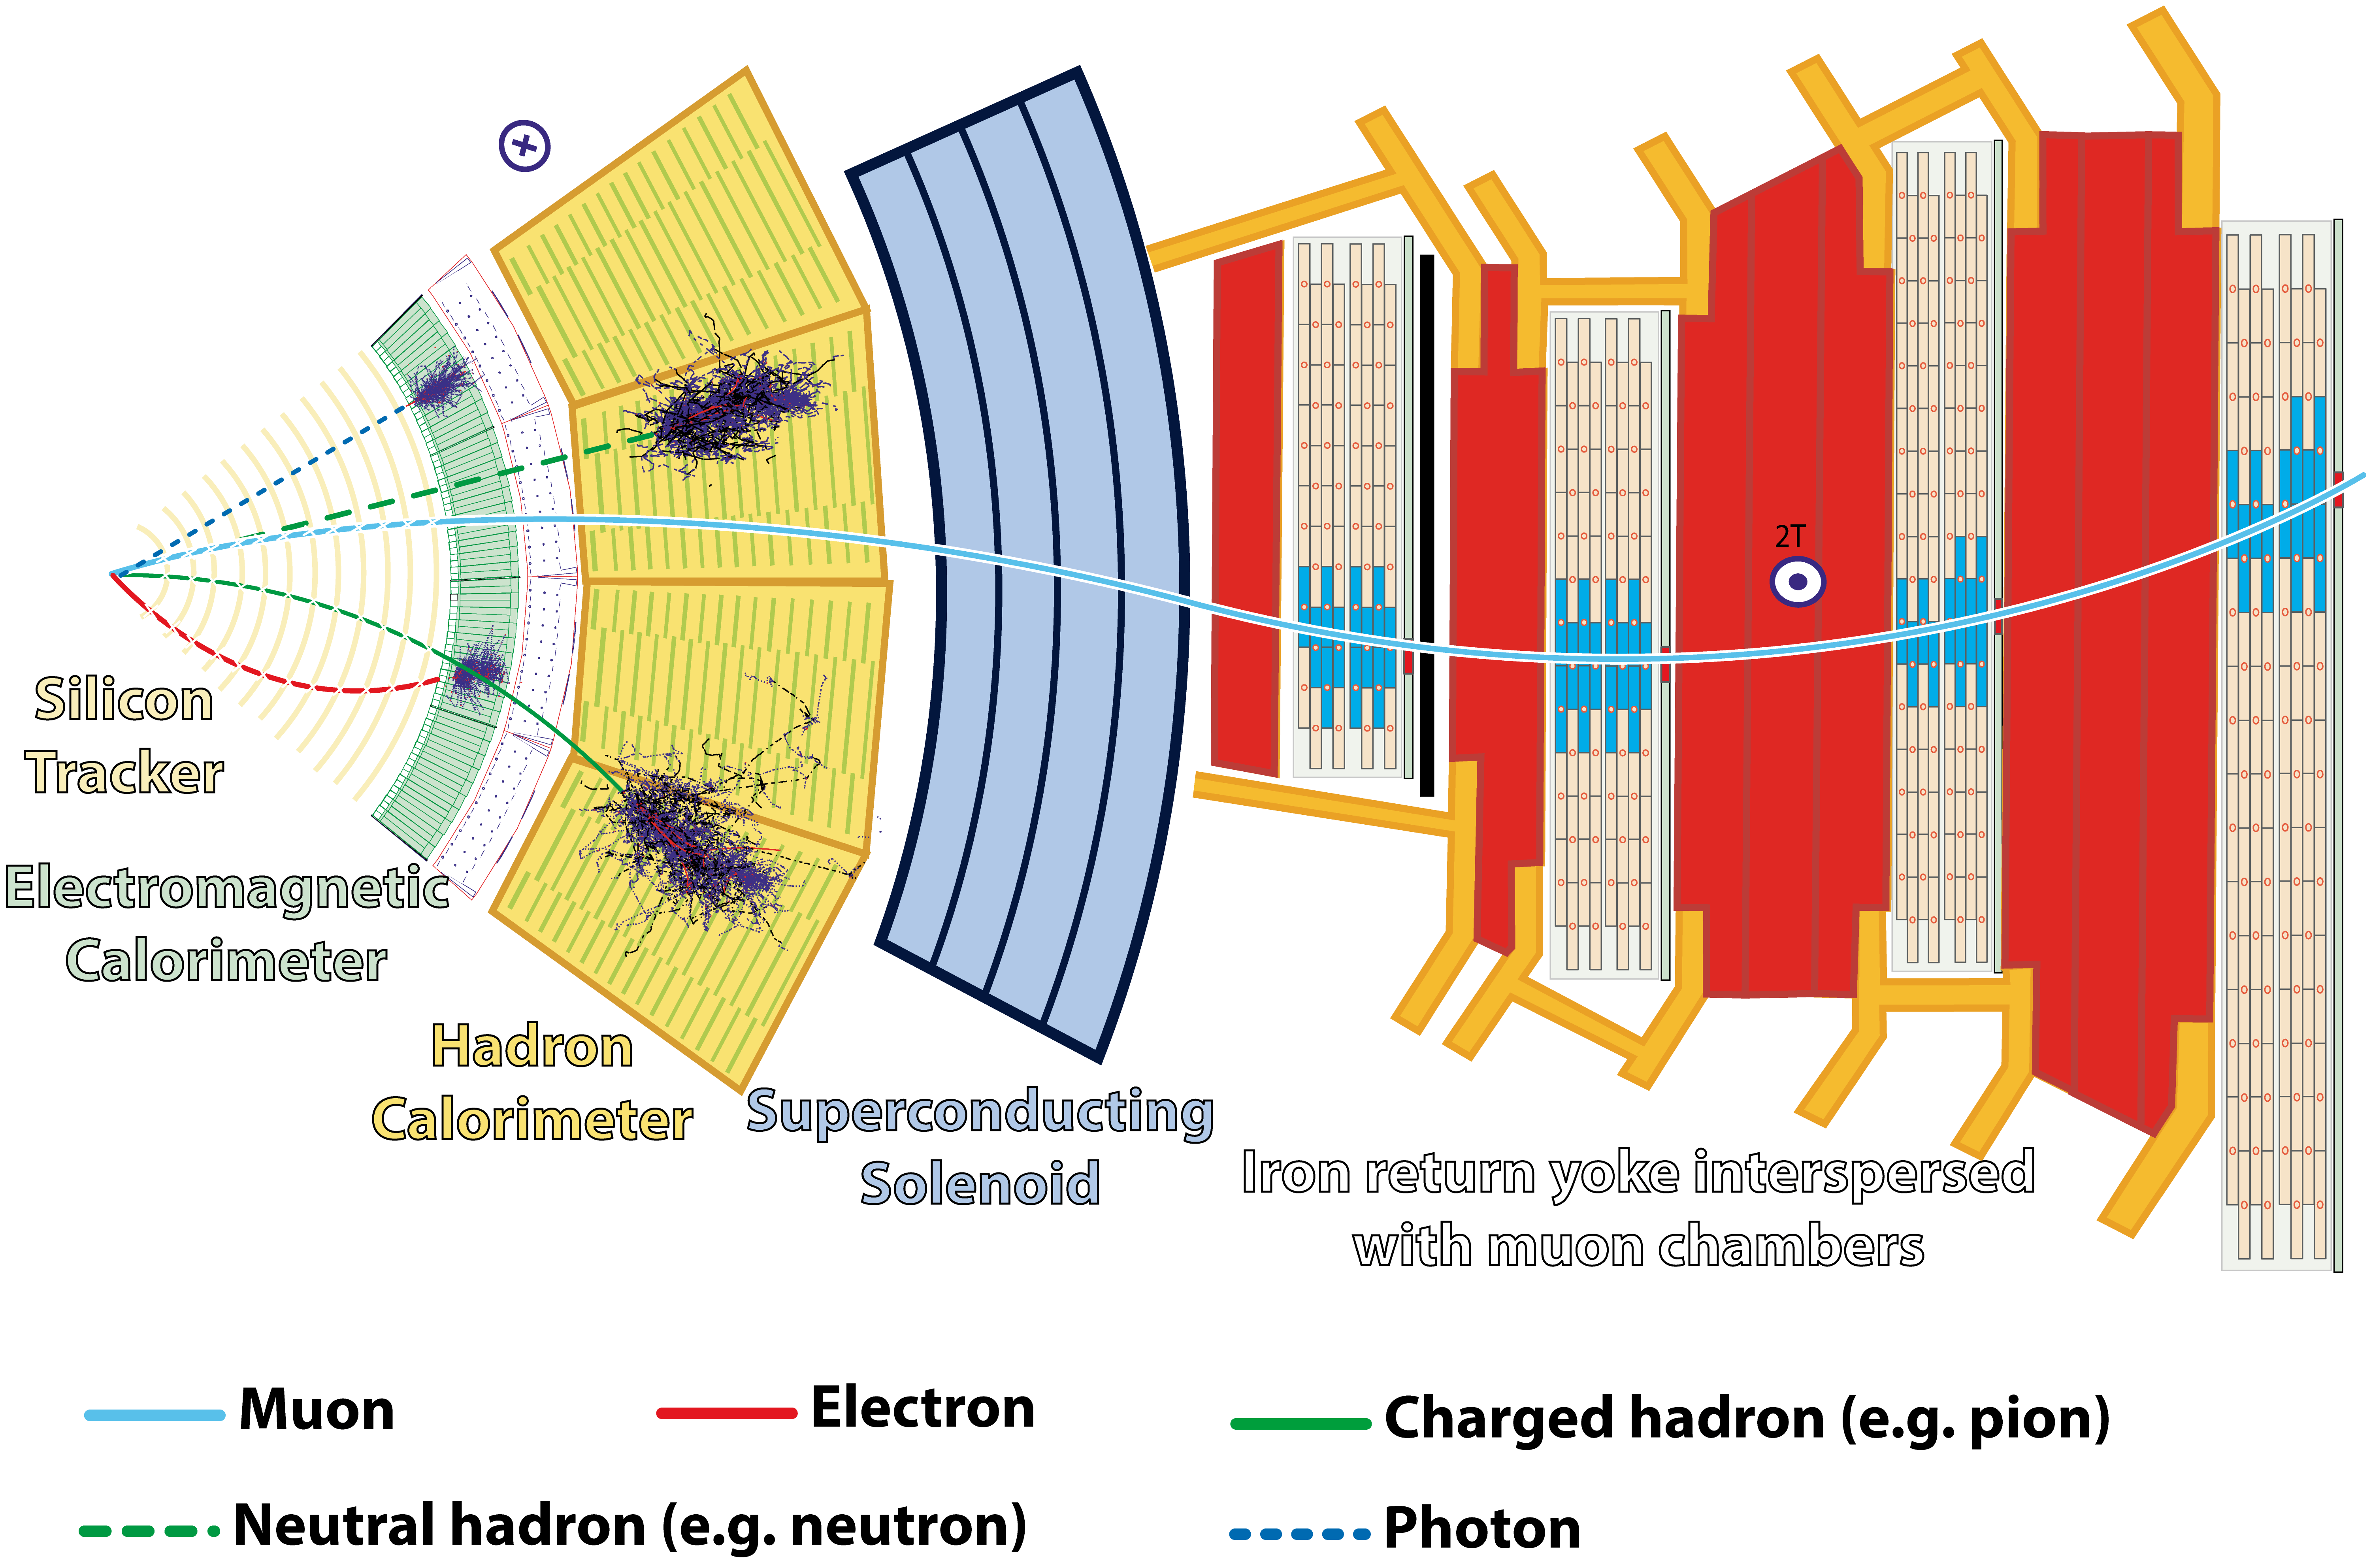
\includegraphics[width=0.56\textwidth]{CMS/particles.png}
	\captionof{figure}{Schéma des traces laissées par différents types de particules dans les sous détecteurs de CMS.}
	\label{particules}
\end{figure}

Les faisceaux ont une fréquence de croisement de 40MHz, chaque événement créer lors de ces collision ont une taille de l'ordre du Méga-octets. Le flux de donnée est bien trop important pour être stocké (~40TB/s). Le flux de données doit donc être réduit, il est donc nécessaire de rejeter des événements afin d'obtenir une fréquence d'acquisition de l'ordre de 300Hz tout en continuant d'enregistrer les événements intéressants pour la physique. Cette étape est réaliser par le système de déclenchement ou \textit{trigger}. La réduction d'un facteur $10^{5}$ de l'acquisition des données est impossible à réaliser en une seule fois, le trigger est donc constituer de deux étapes appelées \textit{Level-1 Trigger} (L1) qui réduit le flux d'événement à 100kHz et \textit{High-Level Trigger} (HLT) qui réduit ensuite ce flux à 300Hz.

\subsection{Le déclenchement de niveau I (L1)}
Le trigger de niveau I (L1) (cf.fig\cref*{L1}) opére à la fréquence de collision des faisceaux (40MHz). L'électronique des détecteurs lisent est stockent les  signaux électriques et les stockent dans une mémoire tampon de 128 événement de collision soit 3.2$\mu s$. Le système de déclenchement possède donc 3.2$\mu s$ pour  décider s'il doit envoyer les données au déclenchement de haut niveau HLT. Chaque 25ns, un nouvel événement rentre dans la mémoire tampon et la décision de garder ou non l'événement arrivé 3.2$\mu s$ plus tôt est prise. Ces 3.2$\mu s$ correspondent à l'envois des données depuis l'électronique des calorimètres et du spectrographe à muons vers la caverne de services qui contient les processeurs gérant la prise de décision, le retour d'un signal pour le rejet ou l'acceptation de l'événement, le délai de synchronisation entre les parties du détecteur ainsi que le tempos de prise de décision. ($\sim1\mu s$). 

	  \begin{figure}[ht!]
	\centering
	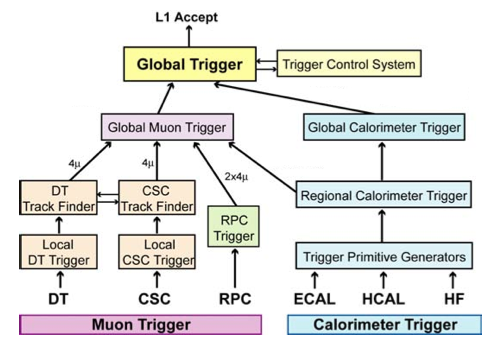
\includegraphics[width=0.70\textwidth]{CMS/L1.png}
	\captionof{figure}{Schéma du L1.}
	\label{L1}
\end{figure}

Chacun des trois sous-détecteur du spectrographe à muons utilise sont propre trigger. Les DT et CSC ont créent des segments de traces. Ces segments sont conservé que s'il pointent vers le point d'interaction. Deux (trois) traces par DT(CSC) sont envoyé au Drift Tube Track Finder (DTTF) (Cathode Strip Chamber Track Finder (CSCTF)) qui cherchent des correspondance entre les traces et assigne un niveau de qualité  au valeur $\eta$ $\phi$ à la charge et à la quantité de mouvement trouvé par ces correspondance et envoie 4 candidat muons au Global Muon Trigger (GMT). Pour le RPC, la sélection est basé sur une coïncidence spatial est temporelle entre les différentes couches. Le Pattern Comparator compare les signaux venant des 4 stations à des patron prédéfini afin de trouver les candidats muons et 8 d'entre eux (4 pour les bouchon 4 pour le tonneau) sont envoyé au GMT. Le GMT reçoit tous ces candidats et combinent ceux trouver dans plusieurs sous-detecteurs. Il assigne ensuite un niveau de qualité à ces nouveau candidats et envois les 4 meilleurs d'enre eux au Global Trigger (GT).

Pour les calorimètre, ils sont réunis en tours de déclenchement qui correspondent aux supercrystaux pour le ECAL. Un candidat est trouvé pour chaque tour du ECAL et HCAL.Le Trigger Primitive Generator est responsable de sommer les énergies venant des différents composant des tours.  Le Regional Calorimeter Trigger (RCT) reçoit les candidats du ECAL et HCAL qui sont répartit en 18 crates qui couvre la moitié des détecteur en $z$ et 40 degree en $\phi$ et fournissent au Global Calorimeter Trigger chacun 4 candidats $e/\gamma$ isolée et 4 candidats non-isolés. Le GCT fournit des informations sur l'isolation et la compatibilité avec des particules d'ionisation minimale au système trigger des muons et classe les candidats $e/\gamma$ par niveau de qualité et envoi les 4 meilleurs isolés et 4 non-isolé au GT. Le GT possèdent également des informations sur les jets, l'énergie transverse totale etc.

La décison finale est faite par le Gloabl Trigger à partir de conditions programmables demandant la présence d'objects ou d'énergie en quantité ou valeurs prédéfinies. Ces conditions forment un chemein de déclenchement. Le Gloabl Trigger permet de programmer et de tester jusqu'à 128 chemins en parallèle. 

\subsection{Le déclenchement de haut niveau (HLT)}
Si l'événement est sélectionné par le L1, il est envoyé au déclenchement de haut niveau (HLT) et les données sont transmises à une ferme de calcul de plusieurs milliers d'ordinateurs  dont chaque processeur exécute le même code de déclenchement (\textit{HLT Menu}) exécuter séquentiellement afin de réduire le temps nécessaire à l'élimination d'un événement et d'améliorer le temps de décision qui doit être de l'ordre de 100ms par événement. Il permet de passer à un flux de donnée de 300Hz. Durant cette phase, les données dui tracker sont utilisés contrairement au L1.

\section{Mises à niveaux et amélioration de CMS}
Le détecteur CMS à déjà subit de nombreuse améliorations depuis le début de sa mise en service (SiPM dans le HO, nouveau trajectographe à pixels...). Cependant, la mise à niveau du LHC vers le HL-HLC prévoit de multiplier la luminosité par $10$, ce qui représente un challenge pour CMS qui doit se mettre à niveau pendant les arrêt LS2 et LS3 afin de pouvoir s'adapter à cette luminosité et au pile-up supplémentaire que cela va engendrer (~140-200 de pile-up). Parmi les mises à niveaux programmées citons \cite{Collaboration:1355706} \cite{Contardo:2020886} :
\begin{itemize}[label=$\bullet$]
	\item Le remplacement des HPD dans les sous-détecteurs HB,HE du calorimètre hadronique pendant le LS2 par des SiPM (comme présent actuellement dans le HO).
	\item Le remplacement complet du trajectographe durant LS3 (cf.fig\ref{tracker2}). La granularité doit être multiplié par 4 afin de gardé une bonne performance de reconstruction malgré l'augmentation du pile-up. Pour cela, les pistes du trajectographe à piste seront raccourcis et le détecteur sera également plus léger afin d'obtenir une meilleur résolution en $p_{T}$ et une conversion des $\gamma$ plus faible. Le trajectographe à pixels aura des pixels et des senseurs plus petit afin d'améliorer la résolution du paramètre d'impact et une meilleur séparation des traces.Plus de 10 disques additionnel dans chaque bouchon seront installé afin de couvrir une zone en rapidité jusqu'à $|\eta|=4$.
	\begin{figure}[ht!]
		\centering
		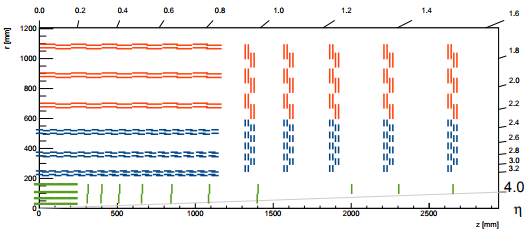
\includegraphics[width=0.85\textwidth]{CMS/tracker2.png}
		\captionof{figure}{Schéma d'un quart du tracker prévu pour la mise à niveau de CMS.}
		\label{tracker2}
	\end{figure}
	\item Les bouchons des calorimètres devront être remplacés par des calorimètre de haute granularité \textit{High Granularity Calorimeter} (HGC) d'une profondeur totale de ~ 10$\lambda$ qui fourniront des images tridimensionnelles détaillées des gerbes. La section électromagnétique est composée d'une trentaine de couches de tungstène et de plaques de cuivre intercalées avec des capteurs de silicium comme matière active. Les capteurs auront des aires variables inférieures à ~ 1,0 cm2. La section électromagnétique fait environs 25X0 et une longueur d'interaction ($\lambda$). La partie hadronique possède 12 plaques de laiton et de cuivre intercalés avec des capteurs de silicium d'une longueur représentant de 3,5$\lambda$ ce qui couvre la majorité d'une gerbe hadronique. Il est suivi d'un "calorimètre hadronique à l'arrière" de conception similaire à l'actuel HE ( des plaques en laiton intercalé avec des carreaux scintillants en plastique lus avec des fibres optiques à décalage de longueur d'ondes). La conception de ce calorimètre à grande granularité s'appuie sur les concepts du ILC / CALICE [21] pour la mesure 3D des gerbes.
	\item le temps de latence du L1 sera augmenté jusqu'à 12.5$\mu s$ ce qui permettra de au système de reconstruction et de d'identification des traces venant des calorimètres et du spectrographe à muons. Pour cela l'électronique de certains sous-détecteurs déjà existent devront être mise à niveau. La fréquence des données en sortie est estimé à 5000Hz(7000Hz) avec 140(200) de pile-up. Le trigger L1 aura également les informations des traces fournit par le trajectographe pour des traces avec $p_{T}\geqq2	Gev$. Ce qui permettra un meilleur pouvoir de rejet du bruit de fond dès le début de la sélection des événements. Un tout nouveau L1 pour les calorimètres et le spectrographe à muons sera également mis en service(cf.fig\ref{L1_2}).
	\begin{figure}[ht!]
		\centering
		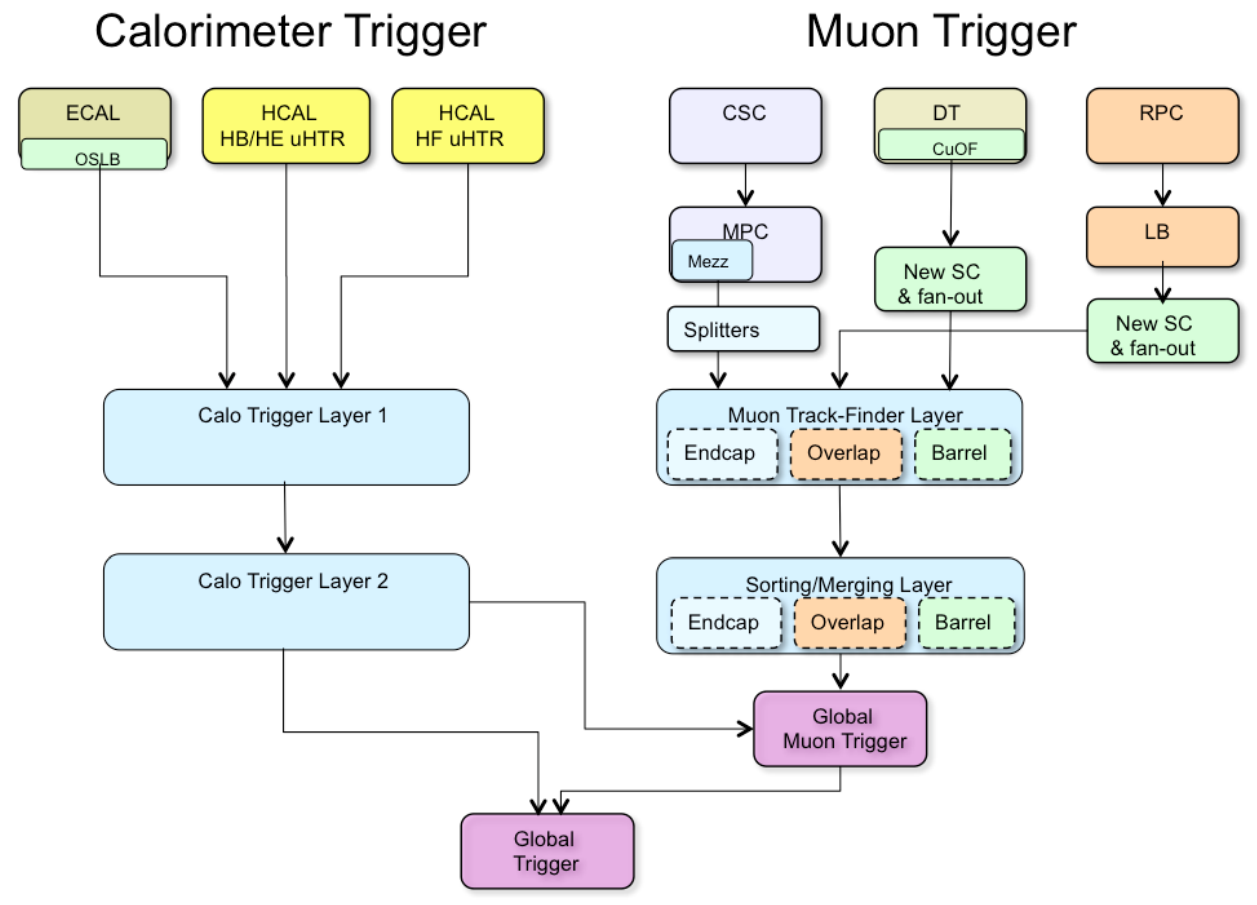
\includegraphics[width=0.60\textwidth]{CMS/L1_2.png}
		\captionof{figure}{Schéma du nouveau L1 pour la partie calorimètre et muons.}
		\label{L1_2}
	\end{figure}
\item Le trajectographe à muons dans le bouchon ne possède que des CSC dans la zone $1.6<\eta<2.4$ actuellement. C'est la seule région du trajectographe qui ne possède pas de RPC afin d'assurer une redondance malgré le fait qu'il s'agissent d'une région dont la résolution de la quantité de mouvement est moins bonne et dont le bruit de fond et important. Afin d'améliorer le L1 dans cette région il est proposé d'instrumenter cette zone avec des chambres de nouvelles technologies. Il est donc prévu d'utiliser des Gas Electron Multiplier (GEM) dans les station ME1 et ME2 qui présente de bonne résolution spatiale et résiste au champ magnétique important présent dans ces zones.Elles permettrons d'améliorer la résolution en quantité de mouvement et d'améliorer la correspondance avec les traces dans le Global Muon Trigger. Pour les deux derniere zone ME3 et ME4, des RPC de meilleur granularité et de bonne résolution temporelle seront utilisées ain de réduire le bruit de fond.  De plus, une nouvelle station ME0 de GEM sera inséré dans l'espace libéré par les nouveaux bouchons de CMS, ce qui augmentera la couverture de détection des muon jusqu'à $\eta\approx3$ (cf.fig\ref{end}). 
	\begin{figure}[ht!]
	\centering
	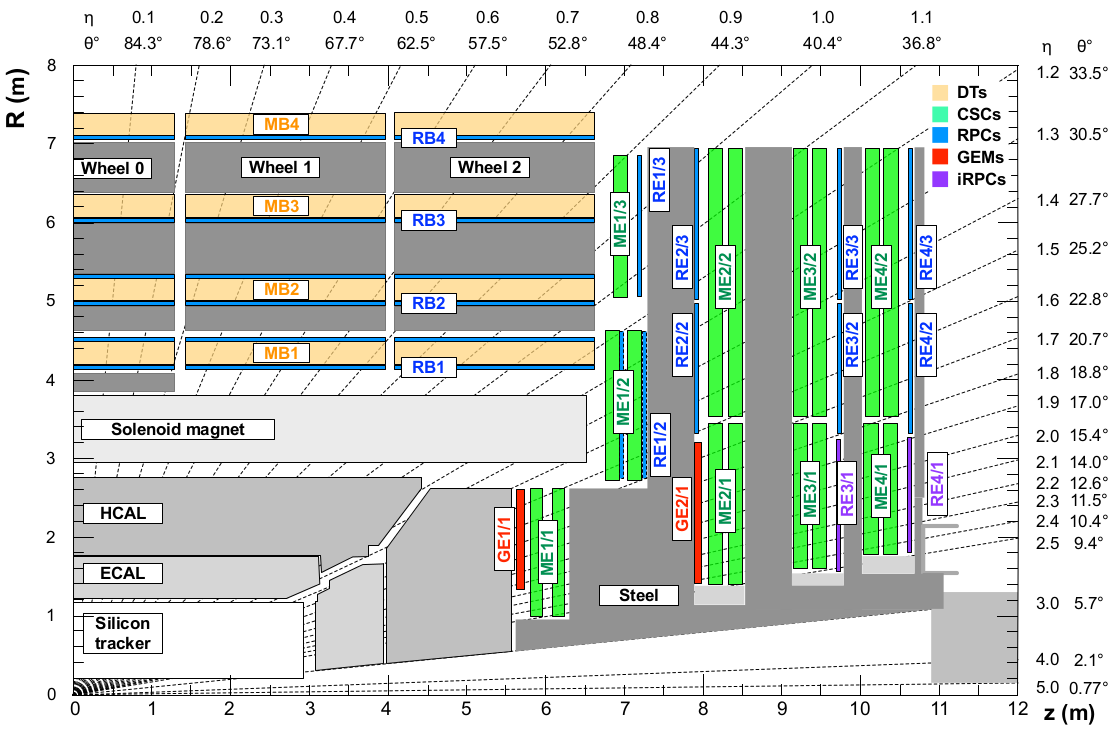
\includegraphics[width=0.60\textwidth]{CMS/endcap.png}
	\captionof{figure}{Schéma d'un quart du détecteur CMS montrant les différentes technologie qui seront instrumentées dans les bouchons.}
	\label{end}
\end{figure}
\end{itemize}
Ce dernier point et plus particulièrement la caractérisation de détecteurs à plaques résistives de verres de basse résistivité est l'objet de cette thèse et sera développé dans les chapitres suivants.